\documentclass[12pt,a4paper]{report}
\setlength\textwidth{145mm}
\setlength\textheight{247mm}
\setlength\oddsidemargin{15mm}
\setlength\evensidemargin{15mm}
\setlength\topmargin{0mm}
\setlength\headsep{0mm}
\setlength\headheight{0mm}

\usepackage[utf8]{inputenc}
\usepackage{graphicx}
\usepackage{epstopdf}
\usepackage{amsthm}
\usepackage{appendix}
\usepackage{nomencl}
\usepackage{parskip}
\usepackage{listings}
\usepackage{enumitem}
\usepackage{nameref}
\usepackage{textcomp}
\usepackage{color}
\usepackage{courier}

\definecolor{lightgray}{rgb}{.95, .95, .95}

\makenomenclature

% Scala listing.
\lstdefinelanguage{Scala}{
  keywords={abstract,case,catch,class,def,%
    do,else,extends,false,final,finally,lazy,%
    for,if,implicit,import,match,mixin,%
    new,null,object,override,package,%
    private,protected,requires,return,sealed,%
    super,this,throw,trait,true,try,%
    type,val,var,while,with,yield},
  otherkeywords={=>,<-,<\%,<:,>:,\#,@},
  sensitive=true,
  morecomment=[l]{//},
  morecomment=[n]{/*}{*/},
  morestring=[b]",
  morestring=[b]',
  morestring=[b]""",
}

% JavaScript listing.
\lstdefinelanguage{JavaScript}{
  keywords={break, case, catch, continue, debugger, default, delete, do, else, finally, for, function, if, in, instanceof, new, return, switch, this, throw, try, typeof, var, void, while, with},
  morecomment=[l]{//},
  morecomment=[s]{/*}{*/},
  morestring=[b]',
  morestring=[b]",
  sensitive=true,
}

\lstset{
	language=Scala,
  backgroundcolor=\color{lightgray},
	basicstyle=\ttfamily,
  keywordstyle=\bfseries,
	extendedchars=true,
	basicstyle=\footnotesize\ttfamily,
	showstringspaces=false,
	showspaces=false,
	tabsize=2,
	breaklines=true,
	showtabs=false,
	frame=leftline,
	captionpos=b,
	frame=single,
	aboveskip=16pt,
	abovecaptionskip=8pt,
}

% Less indented chapter titles.
\makeatletter
\def\@makechapterhead#1{
  {\parindent \z@ \raggedright \normalfont
   \Huge\bfseries \thechapter. #1
   \par\nobreak
   \vskip 20\p@
}}
\def\@makeschapterhead#1{
  {\parindent \z@ \raggedright \normalfont
   \Huge\bfseries #1
   \par\nobreak
   \vskip 20\p@
}}
\makeatother

% Chapter without a number but still in the table of contents.
\def\chapwithtoc#1{
\chapter*{#1}
\addcontentsline{toc}{chapter}{#1}
}

\begin{document}

\lefthyphenmin=2
\righthyphenmin=2



%%%%%%%%%%%%%%%%%%%%%%%%%%%%%%%%%%%%%%%%%%%%%%%%%%%%%%%%%%%%%%%%%%%%%%%%%%%%%%%%
\pagestyle{empty}

\begin{center}
\large Charles University in Prague
\medskip

Faculty of Mathematics and Physics

\vfill

{\bf\Large MASTER THESIS}

\vfill

\centerline{\mbox{\includegraphics[width=60mm]{img/Logo.eps}}}

\vfill

\vspace{5mm}

{\LARGE Jan Široký}

\vspace{15mm}

{\LARGE\bfseries Scala Web Application Toolkit}

\vfill

Department of Distributed and Dependable Systems

\vfill

\begin{tabular}{rl}
Supervisor of the master thesis: & Pavel Ježek \\
\noalign{\vspace{2mm}}
Study programme: & Computer Science \\
\noalign{\vspace{2mm}}
Specialization: & Software Systems \\
\end{tabular}

\vfill

Prague 2013
\end{center}



%%%%%%%%%%%%%%%%%%%%%%%%%%%%%%%%%%%%%%%%%%%%%%%%%%%%%%%%%%%%%%%%%%%%%%%%%%%%%%%%
\newpage
\noindent 
Dedication.



%%%%%%%%%%%%%%%%%%%%%%%%%%%%%%%%%%%%%%%%%%%%%%%%%%%%%%%%%%%%%%%%%%%%%%%%%%%%%%%%
\newpage

\vglue 0pt plus 1fill
\noindent
I declare that I carried out this master thesis independently, and only with the cited sources, literature and other professional sources.

\medskip\noindent
I understand that my work relates to the rights and obligations under the Act No. 121/2000 Coll., the Copyright Act, as amended, in particular the fact that the Charles University in Prague has the right to conclude a license agreement on the use of this work as a school work pursuant to Section 60 paragraph 1 of the Copyright Act.

\vspace{10mm}
\hbox{\hbox to 0.5\hsize{%
In ........ date ............
\hss}\hbox to 0.5\hsize{%
signature of the author
\hss}}
\vspace{20mm}



%%%%%%%%%%%%%%%%%%%%%%%%%%%%%%%%%%%%%%%%%%%%%%%%%%%%%%%%%%%%%%%%%%%%%%%%%%%%%%%%
\newpage

\vbox to 0.5\vsize{
\setlength\parindent{0mm}
\setlength\parskip{5mm}

Název práce: 
Scala Web Application Toolkit

Autor: 
Jan Široký

Katedra: 
Katedra distribuovaných a spolehlivých systémů

Vedoucí diplomové práce: 
Mgr. Pavel Ježek Ph.D, Katedra distribuovaných a spolehlivých systémů

Abstrakt:
TODO

Klíčová slova:
Scala, JavaScript, RIA, JSON, RPC

\vss}\nobreak\vbox to 0.49\vsize{
\setlength\parindent{0mm}
\setlength\parskip{5mm}

Title:
Scala Web Application Toolkit

Author:
Jan Široký

Department:
Department of Distributed and Dependable Systems

Supervisor:
Mgr. Pavel Ježek Ph.D, Department of Distributed and Dependable Systems

Abstract:
TODO

Keywords:
Scala, JavaScript, RIA, JSON, RPC

\vss}



%%%%%%%%%%%%%%%%%%%%%%%%%%%%%%%%%%%%%%%%%%%%%%%%%%%%%%%%%%%%%%%%%%%%%%%%%%%%%%%%
\newpage
\pagestyle{plain}
\setcounter{page}{1}
\tableofcontents



%%%%%%%%%%%%%%%%%%%%%%%%%%%%%%%%%%%%%%%%%%%%%%%%%%%%%%%%%%%%%%%%%%%%%%%%%%%%%%%%
\chapter{Introduction}

The environment of websites and web applications has been rapidly evolving and going through a lot of changes for the last twenty years. It may even be considered the most dynamic area of software development, currently together with mobile application development. The first websites were just static HTML pages linked together with anchors. But people soon found out it is possible to generate the pages on the server, thus provide a dynamic behavior and mimic standard desktop applications. The obvious drawback is that after every action of the user, the whole page has to be reloaded. 

In order to mitigate the problems of dynamic pages, new browser based technologies started to emerge, the most known are Flash\cite{Flash}, Java Applets\cite{JavaApplets} and JavaScript\cite{JavaScript}\cite{EcmaScript}. The proprietary Flash and Java Applets were designed solely for the purpose of web application development, JavaScript was in the first phases meant as a simple scripting language for manipulation with the page. However with the ability to send HTTP requests (known as AJAX\cite{Ajax}), it turned out that JavaScript may be even used as a platform for web applications. 

The current tendency is to move from the proprietary technologies to JavaScript, which is widely supported by browsers and devices. With the new HTML5\cite{Html5} specifications, which are being adopted quite quickly by the major browsers, even the advantages of other technologies (e.g. video in Flash) are disappearing. So a growing number of web applications is in the moment designed as a single HTML page with embedded JavaScript that takes care of everything. And the single page is backed by a server API that the client JavaScript communicates with. This architecture is actually quite similar to the desktop applications, so design patterns and techniques that are already proven-right from the desktop environment may be utilized. From the architectural point of view, the web and desktop application branches are merging.

During past couple of years, JavaScript has been used so extensively, that developers started to reach its limits in modularization and maintainability, mainly while working on big applications. Other programming languages however handle those issues better and because JavaScript is a rather powerful programming language, it is not that difficult to use it as a compilation target for those languages. Even completely new programming languages with the only purpose to improve JavaScript appeared, so currently there is more than one hundred of languages that compile to JavaScript\cite{Backends}, both new and mainstream like Java, C\#, C++ etc.

This approach is actually similar to what happened in the world of standard programming languages, where the bottom level is an assembly language. Other more expressive languages like C or Pascal, which compile to assembler, emerged as soon as an assembly language was not sufficient enough.

\section{Motivation}
\label{sec:Motivation}

The vast amount of compilers targeting JavaScript suggests, there actually are objective reasons and motivation behind them, which drive their development efforts. And because compilation is a development step, that is not present while writing plain JavaScript programs, the motivation has to be strong enough, so programmers are willing to bear this additional step. The following sections should summarize the main disadvantages of JavaScript and briefly describe current trends in the field of JavaScript improving and compilation to it.

\subsection{JavaScript Disadvantages}

When evaluating a programming language, it is always necessary to specify the context of its usage. Here, we are interested in the area of large and complex web applications, so it does not mean that JavaScript should not be used for small and even middle-sized applications.

\subsubsection*{Language} 

The JavaScript itself is a dynamically typed language with prototype-based inheritance, which is rather different from the mainstream enterprise languages. It has no notion of classes, modules, packages or any other such concepts. The whole program consists of bunch of functions and nested objects, which are all accessible from the global scope, due to the fact that object is a key-value table without any access modifiers. There also is not any way how to define interface and its implementation, so it is impossible to hide the complexity of components behind interfaces. All this leads to a drawback, that JavaScript programs are difficult to modularize. Advantages of static typing over dynamic typing are nicely summarized by Erik Meijer\cite{Meijer}: 

\begin{quote}
"...earlier detection of programming mistakes (e.g. preventing adding an integer to a boolean), better documentation in the form of type signatures (e.g. incorporating number and types of arguments when resolving names), more opportunities for compiler optimizations (e.g. replacing virtual calls by direct calls when the exact type of the receiver is known statically), increased run-time efficiency (e.g. not all values need to carry a dynamic type), and a better design time developer experience (e.g. knowing the type of the receiver, the IDE can present a drop-down menu of all applicable members)."
\end{quote}

Even though inheritance is present in JavaScript, it is very different from the class-based inheritance most of the programmers are used to, so it takes some time to fully understand it and take advantage of it. The JavaScript community realizes some of the disadvantages and tries to remedy them on the language level using sometimes peculiar constructs, for example hiding of variables and functions by declaring them as local inside body of an anonymous function which is immediately executed. But there is no standardized or widely adopted way so those efforts stay in the position of suggested conventions.

\subsubsection*{Distribution} 

The most common way of library distribution is one big JavaScript file containing everything. Therefore when a fraction of a library is used, the whole library has to be loaded into the page. And dependencies among the libraries are described in the documentation, so an absence of dependency causes run-time error claiming that a function or an object is undefined. This leads to an environment where the libraries are more likely monolithic and do not share the common functionality even if they could. Similar problem arises when a single application is subdivided into multiple source files. Then all the files have to be declared in the page using script elements in their dependency order. There already exist loaders that handle packaging (most commonly used RequireJS\cite{RequireJs}, HeadJS\cite{HeadJs}) but all share the common disadvantage that the organization of source files into modules and dependencies among them have to be explicitly declared.

\subsubsection*{Development Process} 

As a consequence of the dynamic typing and the fact that field values and thus method implementations are resolved at run-time, some of the processes that can be performed automatically by an IDE or an external tool are not as powerful as in statically typed languages or are even unusable. Because code analyzers and optimizers have much less information about the programs and can not easily reason about them, their power is weaker. But still, there is couple of such tools, e.g. code quality analyzers JSLint\cite{JsLint} and JSHint\cite{JsHint} and code optimizer Google Closure Compiler\cite{GoogleClosure}). Automatic refactoring can not be utilized at all, so in real life it boils down to unreliable operation "replace in files". Intellisense in IDEs is currently at least partially usable however still far behind statically typed languages. Hand in hand with intellisense comes the source documentation in form of documentation comments, because when it does not pop up in the IDE, programmers are less motivated to write it.

\subsection{Improving JavaScript}

When examining current directions of JavaScript improvement, most of them have couple of things in common. They use source languages with static (or at least optionally static) type systems in order to solve the issues related to development process. Moreover, they introduce the concept of packages (or modules, namespaces) for better modularization of programs. All of them switch the prototype-based inheritance for class-based inheritance and together with classes, majority of them also introduces interfaces (or traits, mix-ins) and access modifiers.

So using such a source language that is compilable to JavaScript fixes the aforementioned issues. The problems related to distribution of programs and libraries are mostly handled at the run-time, so it does not affect the source language.

Ideally the source language should be much more expressive than JavaScript, not only small superset in terms of language features, so the compilation step really pays off. Similarly to the step from an assembly language to C, the C language is not just another assembler with some new instructions, but it offers new paradigms, control structures and language constructs that are completely foreign to an assembler.

\subsubsection*{New Languages} 

One branch of the improvement process leads to design of new programming languages solely with the purpose to extend JavaScript. The most well-known examples are Dart\cite{Dart}, CoffeeScript\cite{CoffeeScript} and TypeScript\cite{TypeScript}. Their advantage is that they are designed with the knowledge that programs would be compiled to JavaScript, so for example primitive types don not deviate from JavaScript primitive types. And some of the languages allow optional typing which is good for interoperation with existing libraries. Another benefit is, that from the syntax point of view, they are mostly quite similar to JavaScript so the learning curve is flat for established web application developers. 

On the other hand, the fact they are brand new implies, that for the whole application, one has to be familiar with three programming languages at a time. One for server side, the new language for client side and JavaScript for debugging. Currently both the compilers and browsers start to support source maps which enable debugging in the source language instead of JavaScript, but the the need of knowledge of JavaScript will still be there. 

The type systems of those languages are primitive compared to Haskell, Scala or even C\# and their expressiveness is close to JavaScript. They do not bring any revolutionary concepts, therefore the improvement is not as big as it theoretically could be. From that point of view, CoffeeScript is however the most advanced one.

\subsubsection*{Existing Languages} 

The more appealing idea is to use existing proven language and add the JavaScript backend to its compiler. And if the language is well-suited for web applications or APIs, then even better, because the two ultimate aims could be accomplished: having the whole application written in one language and code-sharing and reuse between server-side and client-side. These goals are so attractive, that the project Node.js\cite{NodeJs} tackles them from the other side by enabling usage of JavaScript on the servers.

Having both sides of the application written in one language even allows implementation of middleware infrastructures, that would support for example remote method invocation known as RPC\cite{Rpc}. That is unthinkable in the plain JavaScript world.

Drawback is that the languages differ from JavaScript a lot, interoperation with it is more inconvenient and in some cases, they are less expressive than JavaScript (e.g. lack of closures in Java). The most famous representatives of this branch are GWT (Google Web Toolkit\cite{Gwt}) for Java and SharpKit\cite{SharpKit} for C\#, but almost all established languages have their JavaScript compilers.

\subsection{Why Scala}

During development of one web application in Scala, whose big part should run in the web browser, it was decided that it would be nice to implement that part using something like GWT, just for Scala. However no such tool turned out to be both usable, maintained and not abandoned. That lead to an origin of the project to implement such a tool for Scala. Later it emerged that it would be more likely a set of tools, therefore the name of the project and also title of this thesis converged to "Scala Web Application Toolkit", shortly "Swat".

Scala is relatively new, yet already established programming language. Among the family of modern programming languages that run on top of Java Virtual Machine (i.e. Scala, Groovy, Clojure, Kotlin) it is the most popular one according to TIOBE index\cite{Tiobe} as of writing this thesis, currently gaining a lot of momentum and being already adopted by commercial companies like Twitter or LinkedIn. Moreover it is backed by strong academic community, so the language with all the concepts and paradigms are well thought through. All these facts determined that it would be good idea to start the project, because there is a possibility for a lot of potential.

\section{Project Aim}

It may be already apparent from the motivation, but the main aim of the project is to create a Scala to JavaScript compiler. From the topmost level point of view, it should take Scala code on the input and produce JavaScript code on the output. The generated code should be somehow embedded or loaded into a web page, so when the page is displayed, it runs and on the algorithmic level does the same thing as if the original Scala code was executed on the JVM. Moreover, it should be possible to access both native JavaScript APIs (e.g. DOM\cite{Dom}, browser-related APIs) and other already existing JavaScript libraries (e.g. jQuery\cite{Jquery}) from the Scala code, in order to manipulate with the web page or with the browser.

With the described setup, it should be possible to take advantage of the fact that both client and server are written in one language and implement simple RPC mechanism. The obvious implication is, that objects would have to be sent through HTTP protocol in both directions and therefore serialized to some common format. To accomplish that, a client side (de)serializer and a server side (de)serializer has to be implemented.

To make the development simple and user-friendly, the tool should be integrated into the SBT (Scala Build Tool\cite{Sbt}) which is currently the most used and to some extent an industry standard in the Scala ecosystem. Moreover, it should be relatively straightforward, to integrate the Swat infrastructure into any web application framework. For the purpose of an example, the web application framework Play\cite{Play} will be used as a reference. SBT and Play are supported by the Typesafe\cite{Typesafe} which is a company founded by the authors of Scala, so both projects are highly maintained with big communities around them.

Finally, a sample application that demonstrates usage of the toolkit should be created. Because the whole toolkit is quite complex piece of software whose size spans behind the scope of this thesis, it is presupposed that not all aspects of it would be fully completed. However the most challenging and difficult parts should be finished. The areas that are not so interesting from the architectural or design point of view would be given lower priority. So the sample application will be rather small.

\subsection{Goals}

To get better understanding, what has to be done, and to somehow break down the project, it is possible to identify couple of steps that have to be analyzed, decided and possibly implemented. The first set of core goals that are critically necessary for the toolkit consists of the following:

\begin{description}[style=multiline,leftmargin=5cm]
\item[1 - Compiler] The Scala to JavaScript compiler and its integration to SBT. It should be the most extensively tested component of the toolkit.
\item[2 - Interoperation] A way how to interoperate with JavaScript APIs and libraries.
\item[3 - Runtime] In case when the generated code is not executable by itself, a runtime that would support the execution.
\item[4 - Libraries] Provide subset of the Scala and Java standard libraries relevant to the web environment.
\item[5 - Integration] Straightforward means of toolkit integration to a web application framework.
\item[6 - Distribution] In the ideal case, a library distribution unit should contain both Scala and the generated JavaScript code.
\end{description}

When the core goals are finished, it is possible to start working on other tasks, that the toolkit in principle could do without. But they bring more comfort to the further development and provide the competitive advantage over other similar tools. The enhancement goals are the following:

\begin{description}[style=multiline,leftmargin=5cm]
\item[7 - Serialization] The serializer \& deserializer usable not only for communication between server-side Scala and client-side generated JavaScript.
\item[8 - Loading] An equivalent to Java classloader that can load compiled JavaScript files from the server on the fly.
\item[9 - RPC] A possibility to mark some methods as remote and infrastructure taking care of the communication.
\item[10 - Application] A sample application.
\end{description}



%%%%%%%%%%%%%%%%%%%%%%%%%%%%%%%%%%%%%%%%%%%%%%%%%%%%%%%%%%%%%%%%%%%%%%%%%%%%%%%%
\chapter{Background}

Both Scala and JavaScript are not mainstream languages in the sense of the chosen paradigms and used concepts, so the following sections will focus mainly on the differences from the conventional object-oriented languages (C++, Java, C\#) and on differences between the two, which are important from the compiler perspective. If you are already familiar with any of the languages, you may skip the corresponding sections. The section \ref{sec:ScalaCompiler} is dedicated to the Scala compiler, its internal processes and related data structures.

\section{JavaScript}

JavaScript\cite{JavaScript} originated as an in-browser scripting language, more recently it expanded to other areas like game-development, desktop applications and server applications. It was designed by Brendan Eich for Netscape, but when it became adopted by other companies, Netscape submitted the language specification to Ecma international which subsequently formalized it in the ECMAScript language standard\cite{EcmaScript}. Regarding syntax and control structures, it was mostly influenced by C and Java, but from the design point of view, the main principles are taken from Self\cite{Self}.

\paragraph{Style} The language is imperative and to some extent functional. It supports standard control structures (e.g. \texttt{if}-\texttt{then}-\texttt{else}, \texttt{while}), makes distinction between expressions and statements, the functions are first-class citizens (i.e. objects themselves that can be manipulated with). One big difference is scoping. Unlike most of the standard languages which have block scoping, JavaScript has lexical scoping. So for example a variable declared inside \texttt{else} branch of an \texttt{if} statement is visible everywhere in the function body.

\paragraph{Type System} JavaScript is dynamically typed, types are associated with values, not variables. The possible types are \texttt{String}, \texttt{Boolean} and \texttt{Number} for primitives, \texttt{Array} for mutable arrays that behave more like hash tables, \texttt{Function} representing functions and methods and \texttt{Object} which is the supertype of all of the aforementioned types. Objects are basically associative arrays, so accessing properties is equivalent to dereferencing values in an associative array by property names. Note that there is not any integral numeric type (e.g. \texttt{int}, \texttt{short}), the \texttt{Number} is a 64bit double-precision floating point type. A character type (\texttt{char}) is not present either.

\paragraph{Inheritance} The most unusual feature is prototype based inheritance, whose principles will be demonstrated on an example of hierarchy \texttt{Dog} \textless: \texttt{Animal} \textless: \texttt{Object} (the "\textless:" symbol stands for the "subtype" relation) depicted on figure~\ref{JavaScriptInheritance}. 

\begin{figure}[ht]
  \centering
	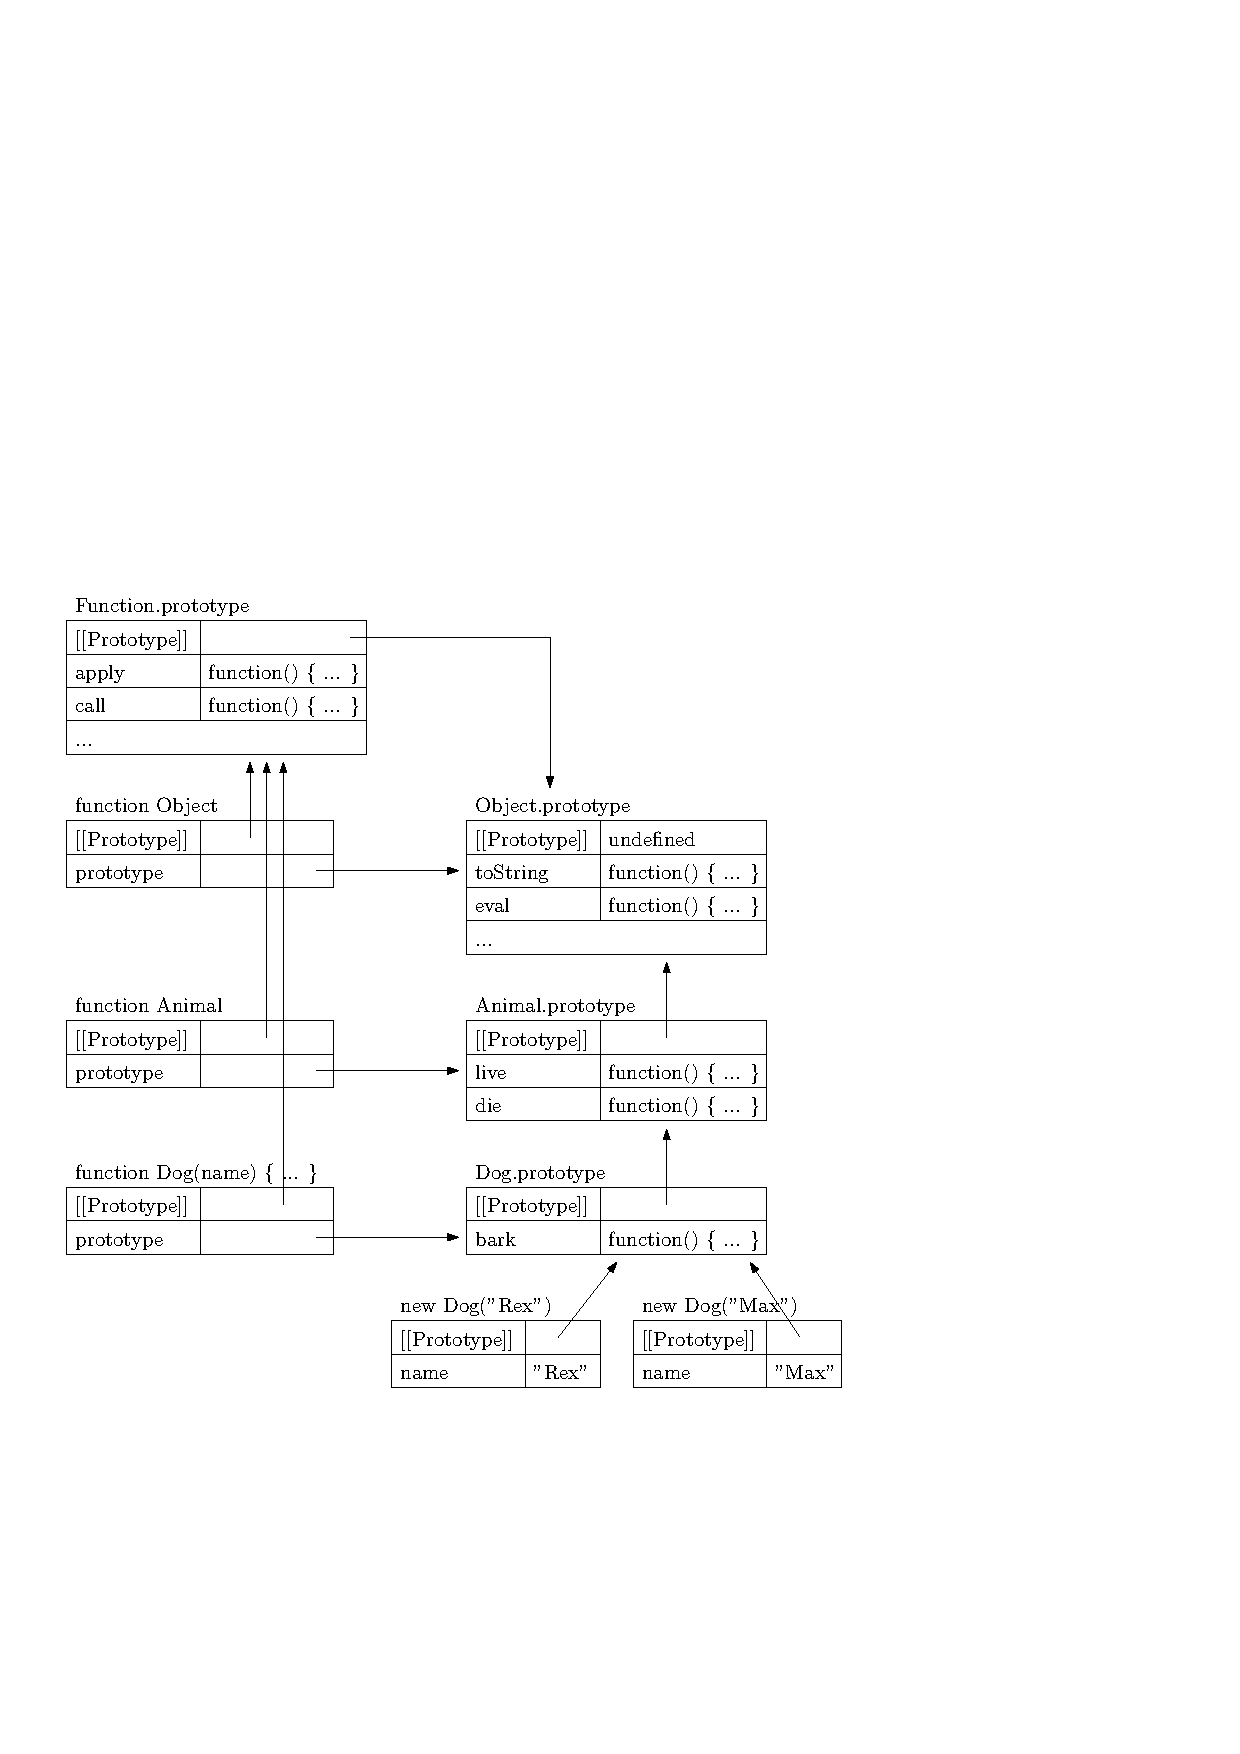
\includegraphics{img/JavaScriptPrototypes.pdf}
	\caption{JavaScript prototypes, constructors and instances.}
	\label{JavaScriptInheritance}
\end{figure}

The first thing to notice is, that all objects (and also functions because functions are objects) have the \texttt{[[Prototype]]} property which holds their prototypes. When a property of an object is being accessed, direct properties of the object are inspected first. If there is no direct property of the specified name, properties of the prototype are inspected. And so on until the prototype of currently inspected object is undefined. As a consequence, it behaves like if the object inherited all properties of its prototype. The \texttt{[[Prototype]]} property is internal, does not change, is assigned once when the object is constructed and can not be changed programmatically.

So for example all functions inherit methods \texttt{apply} and \texttt{call} from their common prototype \texttt{Function.prototype} and transitively methods \texttt{toString}, \texttt{eval} etc. from their prototype's prototype \texttt{Object.prototype}.

In order to create objects, a constructor function has to be defined first (e.g. the function \texttt{Animal} for animals). A constructor function may access the object that is being created via the \texttt{this} keyword and set some of its properties (e.g. the constructor function \texttt{Dog} sets \texttt{name} of a new dog). Moreover it may have associated special object in the property \texttt{prototype} that will be assigned as the \texttt{[[Prototype]]} to all objects created with the constructor function. If the function does not have the \texttt{prototype} specified, the standard \texttt{Object.prototype} is assigned to the created objects. Finally a new object is created by calling a constructor function together with the \texttt{new} keyword, e.g. \texttt{new Animal()}.

To sum it up, the hierarchy on the picture~\ref{JavaScriptInheritance} is set up in the following manner:

\begin{enumerate}
\item Define a constructor function for animals - the function \texttt{Animal}.
\item Assign a new object with properties \texttt{live} and \texttt{die} to the \texttt{prototype} property of the \texttt{Animal} function.
\item Define the dog constructor function \texttt{Dog} with body: \texttt{this.name = name;}.
\item Create a new \texttt{Animal} object (using \texttt{new Animal()}), define it's method \texttt{bark} and set it to the to the \texttt{prototype} property of the \texttt{Dog} function.
\item Create the dogs using \texttt{new Dog("Rex")} and \texttt{new Dog("Max")}.
\end{enumerate}

\paragraph{Environment} JavaScript is an interpreted language, therefore it requires a runtime environment that interprets it and provides objects and functions for the programs interaction with the "outside world". In the context of web applications, both the runtime environment and the outside world is the web browser. The code is executed in a single thread which behaves similarly to an event loop. There is a queue of code that has to be executed. Code is enqueued to the queue from two main reasons: when a new script is loaded and when an external operation handled by the browser finishes and a callback has to be invoked. The environment cyclically waits until the queue is non-empty and then sequentially executes everything in the queue. So it is guaranteed that nothing will run in parallel.

\section{Scala}

One of the best summaries of the Scala language is provided by its author himself, Martin Odersky, in \cite{ScalableComponents}:

\begin{quote}
"Scala fuses object-oriented and functional programming in a statically typed language. Conceptually, it builds on a Java-like core, even though its syntax differs. To this foundation, several extensions are added. From the object-oriented tradition comes a uniform object model, where every value is an object and every operation is a method invocation. From the functional tradition come the ideas that functions are First-class values, and that some objects can be decomposed using pattern matching. Both traditions are merged in the conception of a novel type system, where classes can be nested, classes can be aggregated using mixin composition, and where types are class members which can be either concrete or abstract."
\end{quote}

\paragraph{Style} The language is both imperative and functional, but tends and encourages to use rather the functional style. It supports most of the standard control structures known from e.g. Java. Adds some new control structures, the most important is the \texttt{match} statement (a self explaining example using match is on listing \ref{lst:MatchStatement}).

\begin{lstlisting}[caption={Match statement example.},label={lst:MatchStatement}]
list match {
   case Nil => "empty"
   case 'a' :: tail => "starts with 'a'"
   case (x: Int) :: _ if x > 3 => "starts with int > 3"
   case (x: Int) :: _ => "starts with int"
   case _ => "whatever"
}
\end{lstlisting}

Scala also generalizes existing control structures where it is possible: for cycles are abstracted into much more powerful \texttt{for} comprehensions. The for comprehensions are actually a syntax sugar for series of operations \texttt{map}, \texttt{flatMap} and \texttt{withFilter} whose semantics are defined by the target of their invocation, not by the \texttt{for} comprehension itself. Parallel to that can be found in C\# in the form of LINQ\cite{Linq}, which behaves more less the same. An example of one for comprehension that selects older underpaid employees can be seen on listing \ref{lst:ForComprehension}.

\begin{lstlisting}[caption={For comprehension example.},label={lst:ForComprehension}]
for(e <- employees;
        if e.age > 40;
    c <- companies;
        if c.name == e.companyName;
        difference = e.salary - c.avgSalary;
        if difference < 0		
) yield (e.name, c.name, difference)
\end{lstlisting}

Leitmotif of the Scala language design is a unification of concepts, which appears for example in the \texttt{catch} blocks. Multiple catch blocks for each catched exception type known from standard languages are turned into one that matches against the catched exception. A simple example is provided on the listing \ref{lst:CatchBlock}.

\begin{lstlisting}[caption={Catch block example.},label={lst:CatchBlock}]
try {
    throwsException()
} catch {
    case _: TimeoutException => println("timeout")
    case _: IOException => println("IO")
    case e => println(e.getMessage)
}
\end{lstlisting}

Scala does not differentiate between expressions and statements, because everything, that has been traditionally viewed as a statement (\texttt{if}-\texttt{else}, \texttt{try}-\texttt{catch}), has a return value. So for example a ternary operator is unnecessary, because if-else can be used instead (listing \ref{lst:IfElse}). There are many more features, for a thorough description refer to the Scala "bible" \cite{ScalaProgramming}.

\begin{lstlisting}[caption={\texttt{If}-\texttt{else} as a ternary operator.},label={lst:IfElse}]
val result = if (a >= 0) "positive" else "negative"
\end{lstlisting}

\paragraph{Syntax} As it can be seen on the previous code samples, the syntax resembles Java or C\#, but is much more flexible while trying to reduce unnecessary clutter. It is possible to define methods, whose usage looks like built-in control structures. For example the \texttt{using} syntactical construct known from C\# can be defined in Scala as a library function, whose usage will look exactly the same as in C\#. Leaving out parentheses or semicolons is also allowed in places where they are not necessary. As a consequence, Scala is pretty suitable for design of domain specific languages. 

\paragraph{Type System} Unlike Java with distinct primitive and reference types, where the primitive types do not belong into the inheritance hierarchy, all Scala types inherit from the common ancestor \texttt{scala.Any}. The whole hierarchy is depicted on \ref{ScalaTypeSystem}, the types that are passed by value are descendants of the \texttt{scala.AnyVal}, reference types inherit from the \texttt{scala.AnyRef}. The \texttt{scala.AnyRef} stands for the standard object of the underlying platform, which does not necessarily need to be Java Virtual Machine but also .NET Common Language Runtime. The only non-standard value type is the \texttt{scala.Unit} which represents the product of no types, i.e. the 0-tuple. It has one instance written as empty parentheses - \texttt{()}. The \texttt{scala.Unit} is for example used as a return type of functions that are in other languages defined as \texttt{void}.

\begin{figure}[ht]
  \centering
	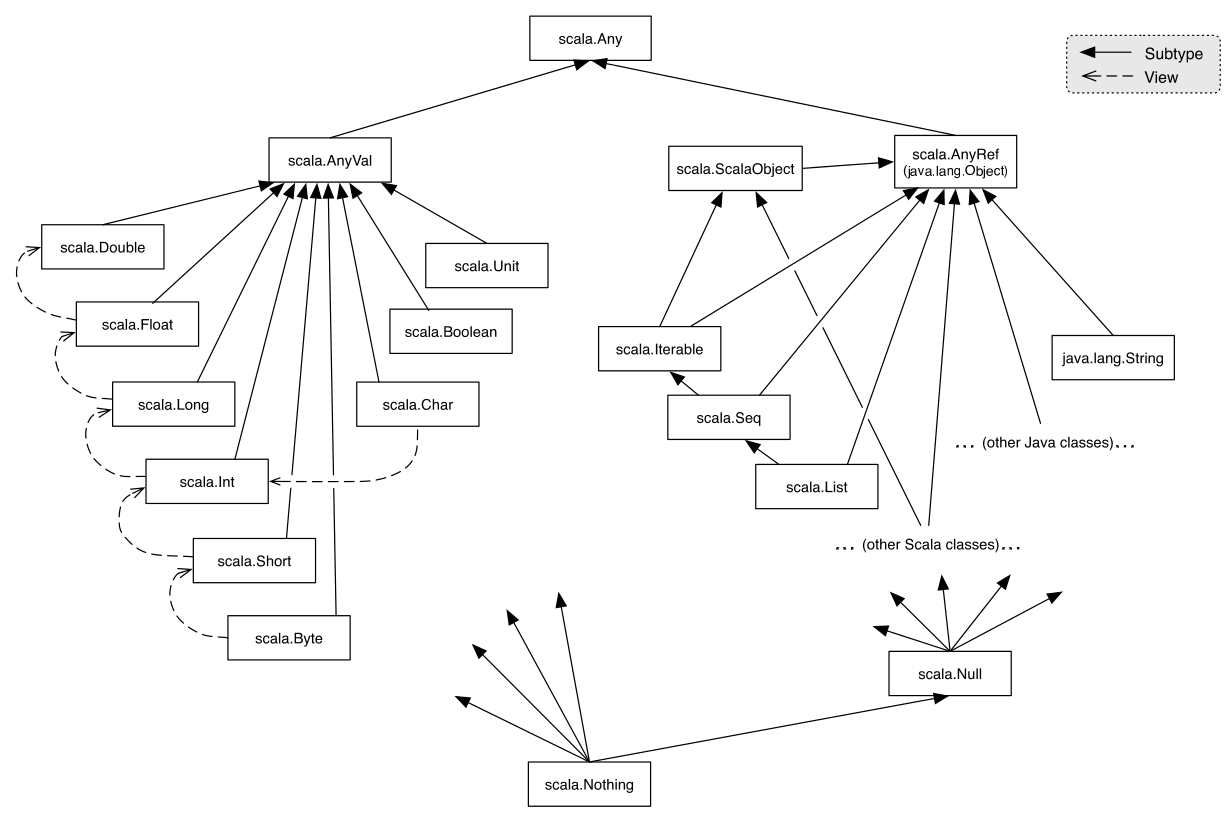
\includegraphics[width=\linewidth,height=\textheight,keepaspectratio]{img/ScalaTypeSystem.png}
	\caption{Scala Type System.}
	\label{ScalaTypeSystem}
\end{figure}

Note the \texttt{scala.Null} type with its only instance \texttt{null} and the uninhabited type \texttt{scala.Nothing} (i.e. no value has such type, in type theory known as the zero type). With them, it is always feasible to determine common supertype and common subtype for each two types\footnote{A common supertype is needed when inferring type of an expression that returns either type A or type B, a common subtype when unifying two generic types with type parameters on a contravariant position.}.

The types may take other types as parameters (known as generic types), the type parameters can be annotated with variance annotations (invariant, covariant, contravariant) and bounded (e.g. the type parameter has to be subtype of type X). Also some more advanced possibilities are supported - existential types, path-dependent types, structural types, etc\cite{ScalaAdvancedTypes}.

\paragraph{Functional Programming} Scala also supports a lot of features that can be found only in functional languages, so it is possible to write Scala programs solely in the functional style. But not purely, because mutable variables, which violate the referential transparency, are allowed. The most important functional concepts are:

\begin{itemize}
\item Closures - anonymous functions that capture the declaration site scope.
\item Immutable variables (\texttt{val}s).
\item Lazy evaluation of variables, function parameters or object fields.
\item Higher-order and nested functions.
\item Currying and partial application.
\item Pattern matching.
\item Tuples and algebraic data types.
\end{itemize}

\paragraph{Object Oriented Programming} On the other hand, Scala is a pure OO language, meaning that every value is an object. A data type may be declared either as a class, a trait or a singleton object. Classes are quite similar to Java classes, but on top of class inheritance, they may mix-in any amount of traits. Traits are basically enhanced Java interfaces with possibility to also define implementation. From the Scala perspective, the only difference between traits and classes is, that traits cannot have parametrized constructors.

The \texttt{static} fields and methods known from mainstream languages are not supported because it is difficult to abstract over them. To fill the gap, singleton objects behave like classes whose only instance is created during the class-loading process. They serve the purpose of static classes but may also inherit or mix-in other types and possibly override something, which is not achievable in languages that use the \texttt{static} modifier.

The famous diamond inheritance problem that always emerges with the multiple inheritance is solved using the technique called linearization\cite{Linearization}. Linearization is a deterministic process that specifies a single linear order for all of the type ancestors (i.e. all classes in the superclass chain and parent chains of all traits). Method resolution takes advantage of it and works in the linearization order, so there is no place for ambiguity left.

\section{Scala Compiler}
\label{sec:ScalaCompiler}

In the context of the thesis, it is also important to know how the Scala compiler works, because it may be used by the Swat as a library for tasks that are specific for Scala compilation, but not that relevant from the Scala to JavaScript compilation perspective. The compiler architecture is summarized by Martin Odersky in \cite{ScalableComponents}:

\begin{quote}
"The Scala compiler, \texttt{scalac}, consists of several phases. The first phase is syntax analysis, implemented by a scanner and a conventional recursive descent parser. The result of this phase is an abstract syntax tree. The next phase attributes the syntax tree with symbol and type information. This is followed by a number of phases that transform the syntax tree. Most transformations replace some high-level Scala-specific constructs with lower-level constructs that can more directly be represented in bytecode. Other transformations perform optimizations such as inlining or tail call elimination. Transformations always consume and produce attributed trees."
\end{quote}

So the compiler can be understood as a sequence of phases where each phase takes an abstract syntax tree (AST) as its input from the previous phase, adds attributes to the AST or modifies the AST and passes the modified tree to the consequent phase.

In order to represent a scala program in the compiler, a couple of data structures needs to be defined\cite{Reflection}
. \texttt{Name}s represent identifiers that appear in the source code, e.g. class names or field names. \texttt{Symbol}s are used to bind a name and the entity it refers to, such as a class or a method. Anything that can be given a name has a symbol associated with it. Instances of the \texttt{Type} class represent information about the type of a corresponding symbol (the information include member methods, fields, base types etc). Finally, the ASTs are represented by \texttt{Tree} and its subclasses that correspond to various source code elements such as class definitions (\texttt{ClassDef}), method invocations (\texttt{Apply}) or \texttt{if}-\texttt{else} statements (\texttt{If}).

The only up-to-date description of the phases, the scalac consists of, can be found in the source code (class \texttt{scala.tools.nsc.Global}). Here are the most important ones in their execution order:

\begin{description}[style=multiline,leftmargin=5cm]
\item[\texttt{syntaxAnalyzer}] Takes Scala code as its input, parses source code into ASTs, performs simple desugaring.
\item[\texttt{namerFactory}] Declares symbols and enters them into scopes
\item[\texttt{typerFactory}] Assigns types to symbols, the most complex phase.
\item[\texttt{patmat}] Converts the \texttt{match} expressions into if-else statements, labels and jumps.
\item[\texttt{uncurry}] Performs the opposite of currying, transforms variadic parameters to sequences, converts closures to anonymous classes and a lot of other similar, rather simple, operations. 
\item[\texttt{explicitOuter}] For each nested class, adds a field for the reference to the outer class instance. 
\item[\texttt{erasure}] Erases generic types, adds interfaces for traits.
\item[\texttt{lambdaLift}] Move nested function definitions to the top level.
\item[\texttt{lazyVals}] Converts lazy fields into methods.
\item[\texttt{constructors}] Moves field initialization into constructors.
\item[\texttt{mixer}] Performs the mix-in composition.
\item[\texttt{cleanup}] Platform specific cleanup.
\item[\texttt{deadCode}] One of many optimization phases, eliminates dead code.
\item[\texttt{jvm}] Generates the Java bytecode.
\end{description}



%%%%%%%%%%%%%%%%%%%%%%%%%%%%%%%%%%%%%%%%%%%%%%%%%%%%%%%%%%%%%%%%%%%%%%%%%%%%%%%%
\chapter{Analysis}
\label{sec:Analysis}

This chapter proposes, how some of the defined goals can be fulfilled, while providing more possibilities with their pros and cons. It should not be biased by the fact, that the source language is Scala, so the described methods could be applied even in a different environment. But for example purposes, Scala will be used, because it is the source language of the Swat. Moreover, this chapter elaborates on which of the proposed approaches is used by the Swat and why.

\section{Setup}

Compiler architecture has converged throughout years to a data flow consisting of canonical components. The source code is consumed by a scanner, that performs lexical analysis and produces a stream of lexical tokens. A parser takes the token stream on the input, performs syntactical analysis and builds up the ASTs. The ASTs are then processed by a semantical analyzer which validates them, assigns types to symbols and possibly transforms the ASTs. These three components are marked as the frontend components. When the abstract syntax trees leave the frontend, they go to a backend, which is responsible for generation of the target language/assembly/byte code. The backend usually consists of several subcomponents that firstly produce some intermediate code, optimize it and then generate the machine specific code. Such a data flow can be seen on the the picture \ref{Compiler}.

\begin{figure}[ht]
  \centering
	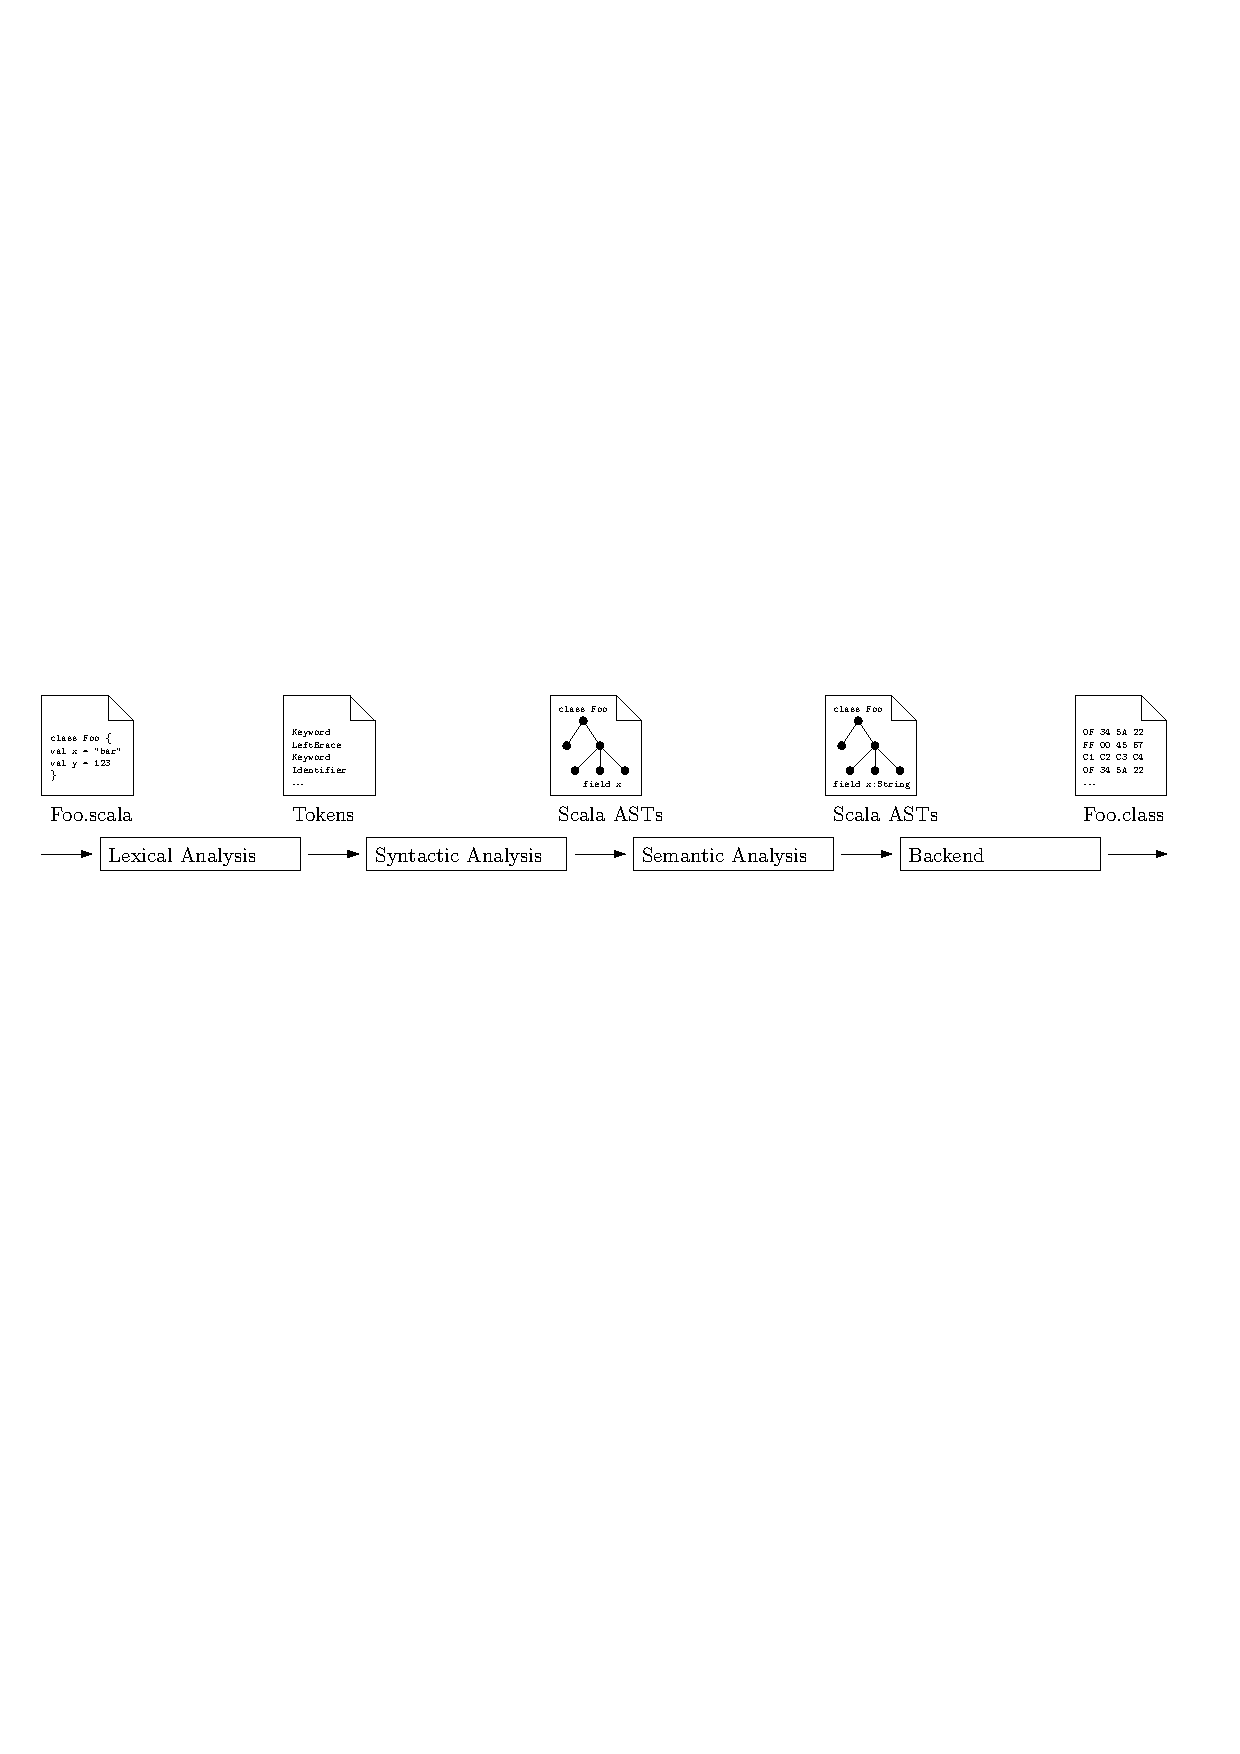
\includegraphics[width=\linewidth,height=\textheight,keepaspectratio]{img/Compiler.pdf}
	\caption{Canonical compiler architecture.}
	\label{Compiler}
\end{figure}

In order to transform programs to JavaScript, one needs to work with them programmatically. ASTs exactly serve this purpose and because standard compilers (e.g. javac, csc, scalac) already handle the transformation from source code to ASTs, reusing that functionality is definitely the way to go.

\begin{figure}[ht]
  \centering
	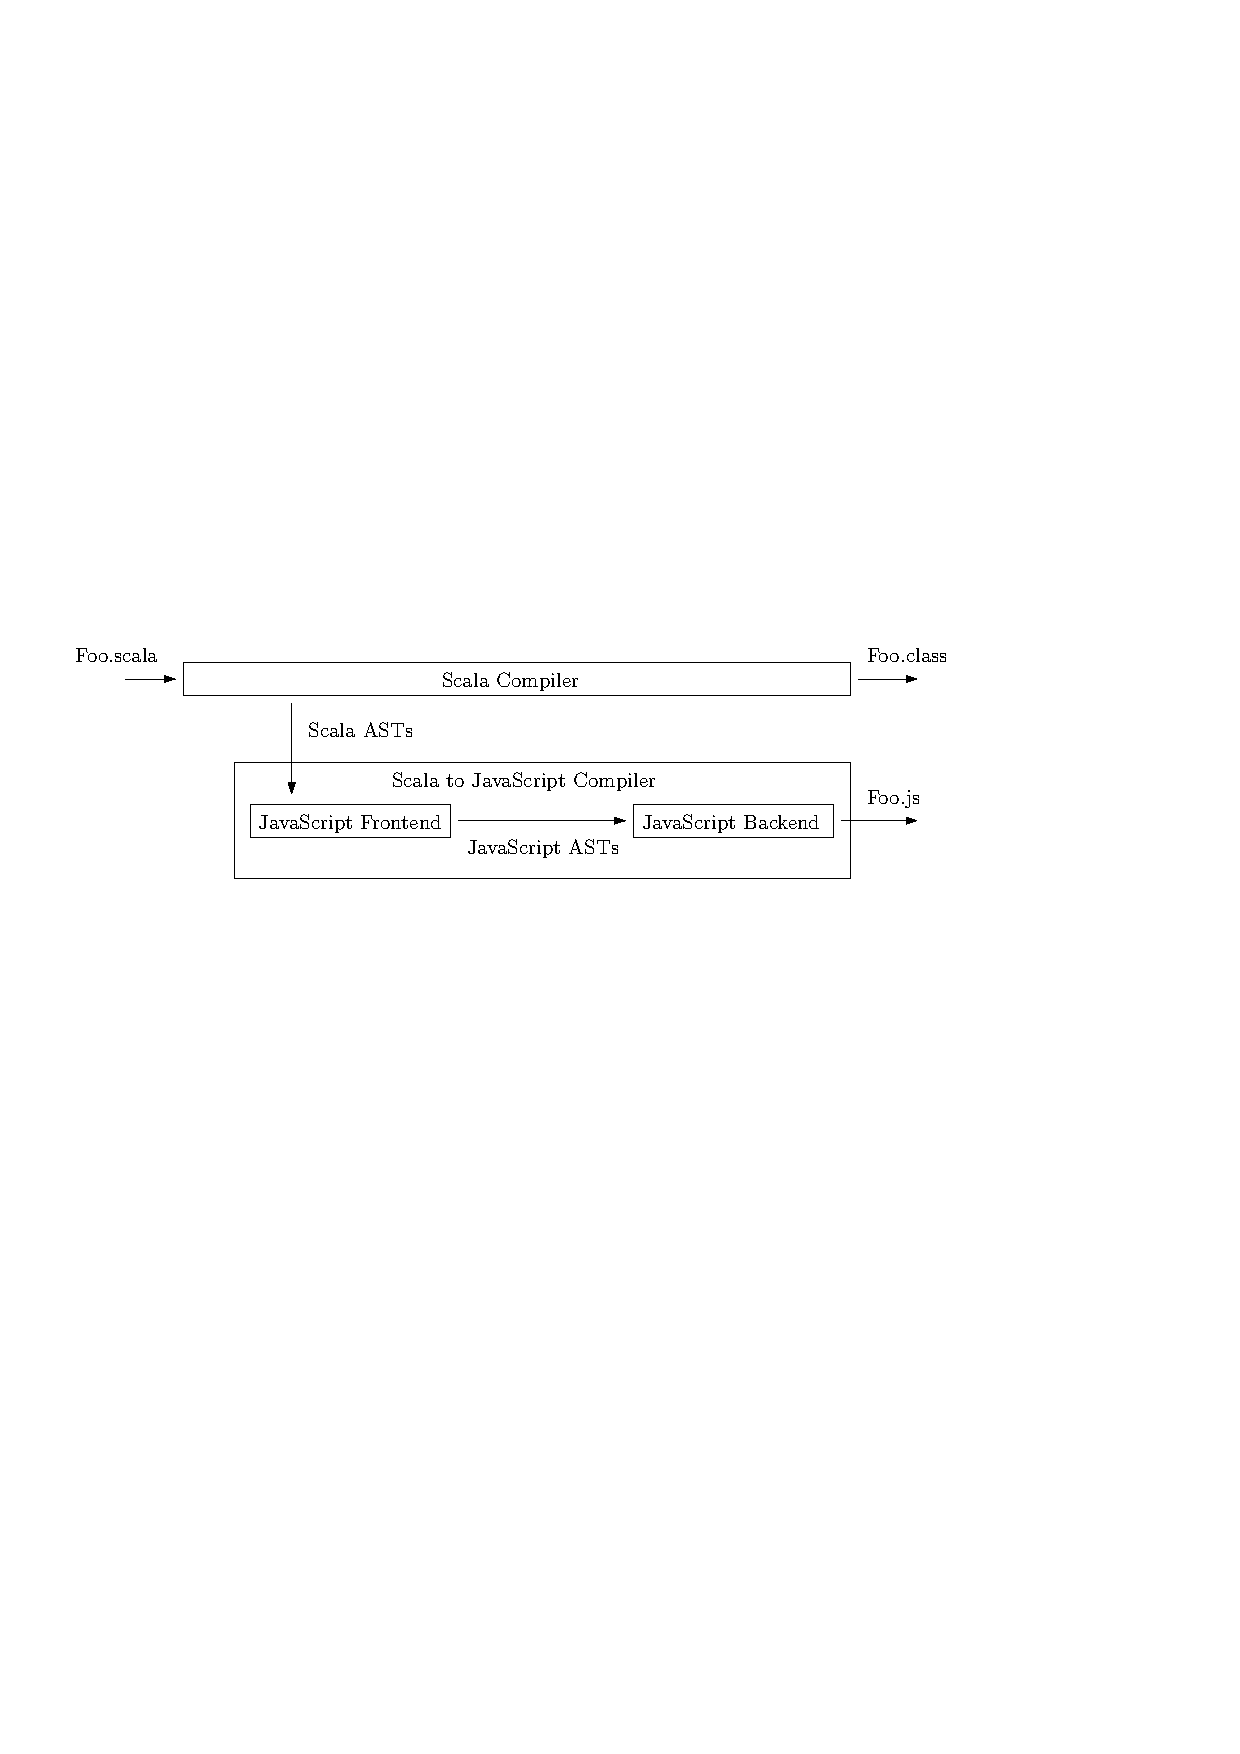
\includegraphics[width=\linewidth,height=\textheight,keepaspectratio]{img/CompilerPlugging.pdf}
	\caption{JavaScript compiler using the source language compiler.}
	\label{CompilerPlugging}
\end{figure}

As it can be seen on the diagram of the whole setup (figure \ref{CompilerComplete}), the compiler to JavaScript itself follows the canonical structure, therefore it consists of a frontend and a backend. The JavaScript Frontend in ideal case consumes ASTs obtained from the source language compiler and produces corresponding JavaScript ASTs. When the JavaScript frontend is done, the execution proceeds to the JavaScript Backend. It generates JavaScript code corresponding to the ASTs and may optimize the output either by itself or by an external tool (Google Closure compiler\cite{GoogleClosure} is the most popular JavaScript optimization tool).

Another advantage of the proposed setup is, that compilation to bytecode and compilation to JavaScript is performed during one run of the composed compiler, mainly because the time for lexical analysis, syntactical analysis and possibly type checking is spent only once. And it is common knowledge, that these three operations take the most of the compilation time. One may also ask, why the compilation to bytecode is necessary after all. The main reason is, that when a library compiled to JavaScript is used by a different project compiled to JavaScript, then compilation of the different project passes only if the library classfiles are on the compilation classpath. The other reason is simply code sharing between server side and client side.

\subsection{Utilizing the Source Language Compiler}

The standard compiler architecture offers a few places where the ASTs can be obtained. As depicted on the figure \ref{Compiler}, it is either before the semantic analysis is executed (option A) or after execution of the semantic analysis (option C). If the compiler components are subdivided into phases, it may be even possible to access syntax trees during execution of the semantic analysis (option B). That mostly depends on architecture of the source language compiler, whether it allows such an interception.

\begin{figure}[ht]
  \centering
	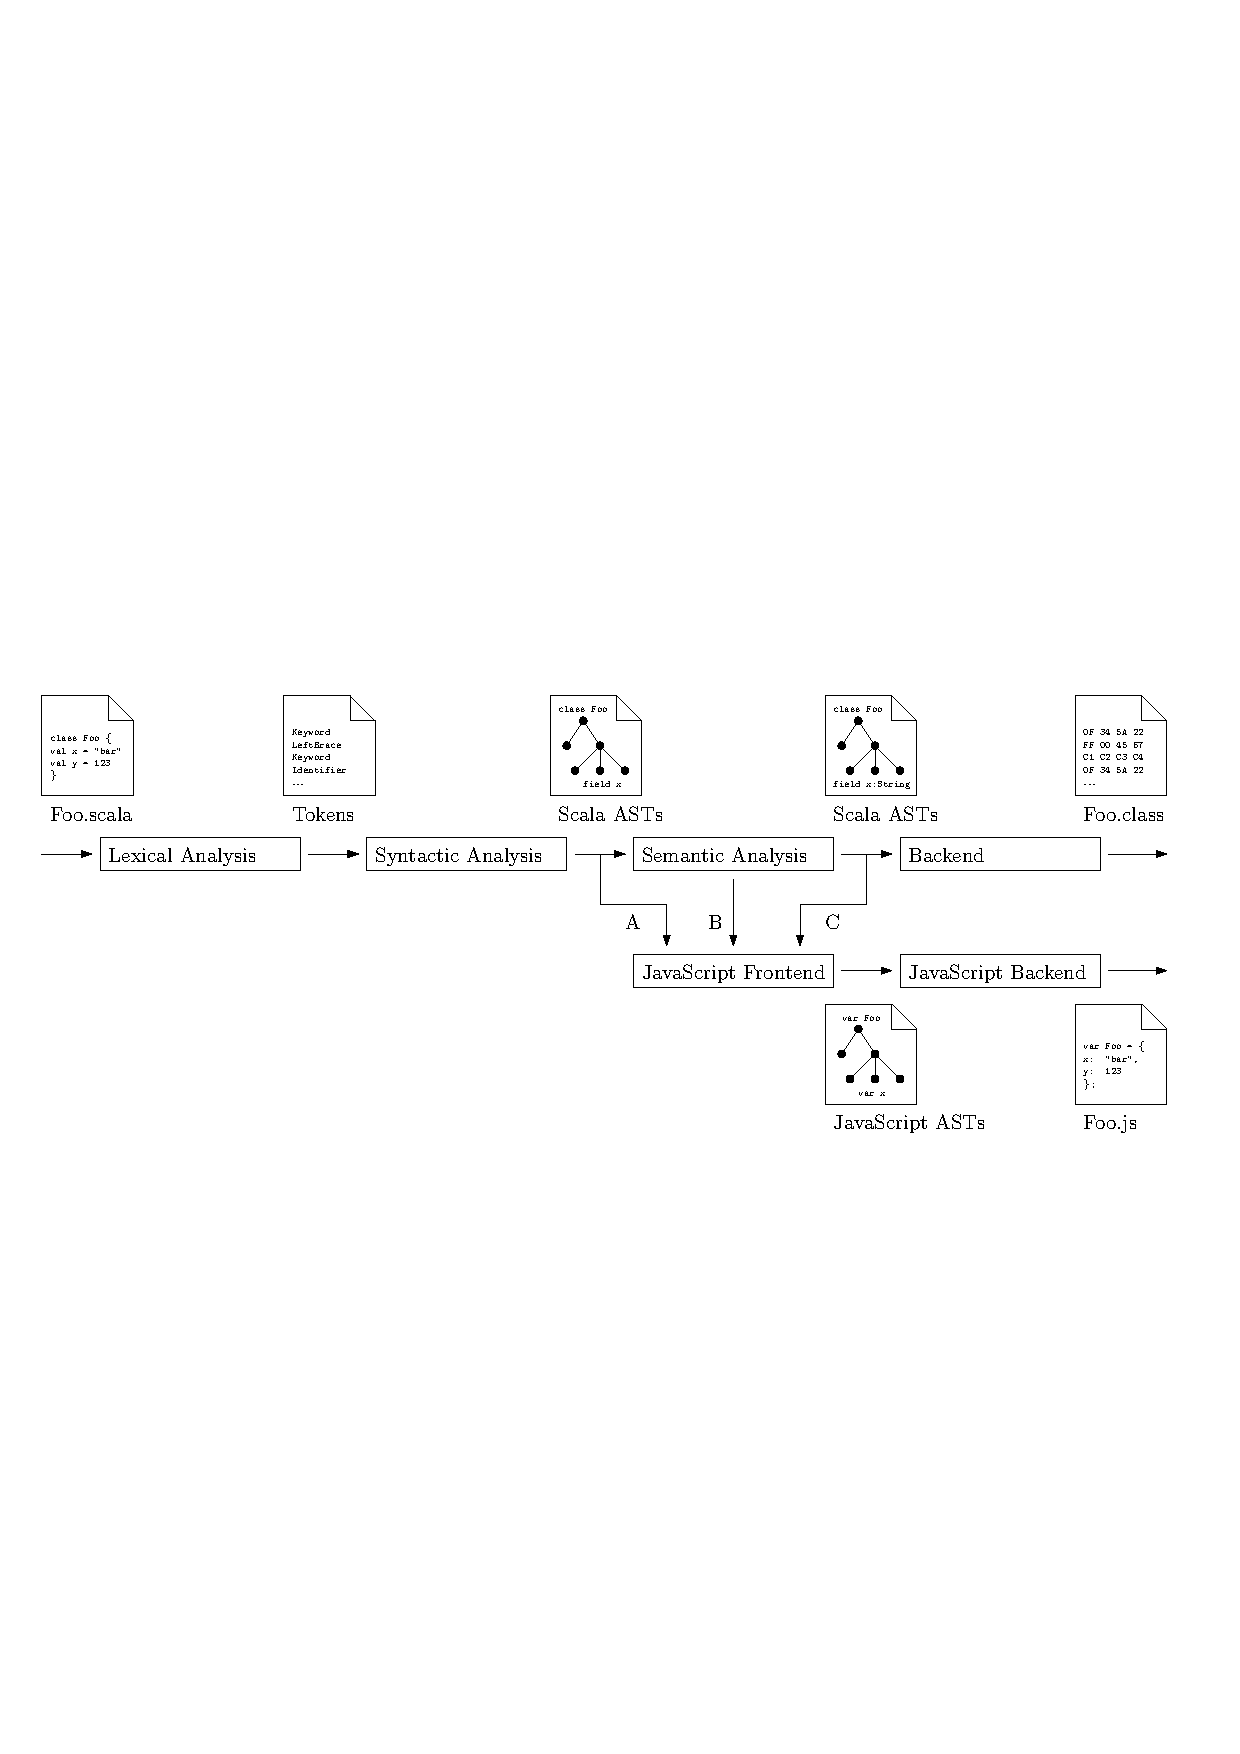
\includegraphics[width=\linewidth,height=\textheight,keepaspectratio]{img/CompilerComplete.pdf}
	\caption{Plugging JavaScript compiler into source language compiler.}
	\label{CompilerComplete}
\end{figure}

Choice between options A, B and C determines abilities of the JavaScript frontend. The ASTs may just mirror the source code with no added information (option A), they may be completely analyzed and possibly transformed to some extent (option C), or the ASTs may be in an interim state between A and C (option B). An issue with the option C is, that some of the trees may be transformed to constructs that are really low-level and close to bytecode, even though the original trees would be directly expressible in JavaScript before the transformation.

The Scala compiler is subdivided into phases so the most crucial decision is finding the spot where the compiler to JavaScript should be plugged in. Scala compiler phases have fixed order and dependencies and it is almost impossible left out a phase from the sequence. So the decision is where to cut the sequence into two parts.

Principally the compiler to JavaScript could be plugged anywhere. The earlier it is plugged in, the more work for it because the early phases work with much richer set of tree types compared to the latter phases where some of the AST types are completely eliminated (e.g. \texttt{Match} by phase \texttt{patmat}). On the contrary the ASTs that appear on the beginning of the phase sequence practically mirror the original Scala code whereas the ASTs towards the end look more like Java mixed with bytecode.

One of the aims was to produce JavaScript code that would resemble Scala as much as possible and use just the compiler phases that analyze the code (\texttt{syntaxAnalyzer}, \texttt{namerFactory}, \texttt{typerFactory}). The motivation behind it was to simplify debugging of the compiled code in a web browser. But it turned out that it would be a lot work to implement JavaScript counterparts of Scala control structures that are not present in JavaScript. So the phases \texttt{patmat}, \texttt{uncurry} and \texttt{explicitOuter} should also be utilized, because they transform higher level Scala constructs to ones that are directly expressible in JavaScript. From the other point of view, the phase \texttt{erasure} does not bring any added value in the context of compilation to JavaScript, it erases some of the type information. The phases after \texttt{erasure} (namely the \texttt{lamdaLift}) transform the trees to an extent, that is not acceptable if the resulting JavaScript code should resemble Scala at least a bit. To sum it up, the place between \texttt{explicitOuter} and \texttt{erasure} is where the Swat compiler should be plugged in.

\subsection{Debugging}

The chosen plugging place implies that the resulting code sometimes would not resemble the source Scala code, which means that debugging the program directly in JavaScript in a web browser would be tricky. This way of debugging is not ideal even if the outputted JavaScript code looked almost the same as the source it was compiled from. Similar problem appears in the plain JavaScript world where code that went through minification (e.g. whitespace removal, name shortening) is difficult to debug.

JavaScript ecosystem and web browsers offer a solution in form of source maps\cite{SourceMaps} that establish mapping between the executed JavaScript code (minified or compiled) and the original code (not minified or even possibly not JavaScript) and allow a user to debug the original code. Source maps are still state of the art functionality not supported by all browsers and establishing such a mapping can be quite complex task, so the implementation of it is behind the scope of the thesis.

\section{Interoperation with JavaScript}

One of the crucial requirements of a compiler targeting JavaScript is enabling the programs written in a source language to interoperate with the JavaScript environment. A reason for it is that the programs do not run in a vacuum and the only possibility how they can manifest themselves is via interaction with the hosting environment. It is feasible to make interoperation with the environment type safe, because the APIs are defined mostly in W3C\cite{W3c} specification with types included. It is JavaScript where the type information is lost. Another reason is that sometimes it makes sense to descend to the JavaScript level and write a piece of code directly in it, for example for performance reasons. 

Inherent restriction of the interoperation is that the used solution should not violate syntax of the source language. There are several ways how to accomplish the proposed requirements, the following three solutions represent different ways of doing it and are more less orthogonal to each other: 

\paragraph{Native code blocks} A parallel to the inline assembler blocks in the C language, with difference that the JavaScript code has to be placed in a string in order not to violate the source language syntax. Moreover type of the whole code block expression (e.g. \texttt{js("123 + 456")}) has to be \texttt{scala.Nothing} so it can be used even in places where a value of particular type is expected. When the JavaScript Frontend encounters such a block it outputs only the code stored in the string. Example of such a code block can be seen on the listing \ref{lst:NativeCodeBlock}.

\begin{lstlisting}[caption={Native code block example.},label={lst:NativeCodeBlock}]
def repeat(text: String, times: Int): String = js("""
  var a = [];
  while(a.length < times) {
    a.push(text);
  }
  return a.join('');
""")
\end{lstlisting}

\paragraph{Adapters} For all the JavaScript APIs and objects that should be usable from the source language, so called "adapter" classes are defined in the source language. They should exactly match the JavaScript definitions in terms of names, fields, methods, parameters etc. and should be marked with an annotation in order to be distinguishable. They do not have to be implemented, but the type signatures should match the specification (see the listing \ref{lst:Adapters} where an adapter for the \texttt{window} object is defined and used). When the compiler encounters such an adapter class, it knows that it is something that is already present in the JavaScript environment, so it can be completely ignored.

\begin{lstlisting}[caption={Adapter definition and usage example.},label={lst:Adapters}]
@adapter object window {
  def alert(text: String) {}
}

def test() {
	window.alert("test")
}
\end{lstlisting}

\paragraph{Dynamic} This option is relevant only to source languages that support the concept of a dynamic class. In Scala, an object named \texttt{global} representing the JavaScript global scope (\texttt{object global extends Dynamic}) is defined. The object mixes-in the \texttt{scala.Dynamic}\cite{ScalaDynamic} trait, so any field can be selected or any method can be invoked on that particular object. For example \texttt{global.window} will be turned by the Scala compiler before the typing phase into \texttt{global.selectDynamic("window")}. Such an invocation can later be transformed by the JavaScript Frontend into \texttt{window}.

As it was mentioned in the motivation, static typing is an advantage in the context of large applications, so the option {\it Adapters} is the preferred one. Unlike the two other, it preserves type safety. The tradeoff is that it is incomparably more time-consuming for a developer to define all the adapters compared to the other options where nothing has to be declared. For exceptional purposes (performance optimization) the {\it Native code blocks}, which are more flexible than than {\it Dynamic} could be used.

\section{Frontend}

A heart of the whole Swat toolkit is the JavaScript frontend responsible for transformation of source language ASTs to JavaScript ASTs. It starts given the whole program in the form of a syntax tree, traverses the AST and produces a JavaScript AST. According to the current subtree, whose root the fronted is visiting, it should produce JavaScript counterpart for that subtree. The following sections describe options the fronted has and elaborate on how particular tree types should be represented in JavaScript. It is natural to start with the top-level node that encapsulates everything else and traverse down the tree through class definitions, their member definitions to the simplest expressions on the leaf level of the tree.

\subsection{Compile Time vs. Runtime Approach}

The JavaScript frontend can use different approaches to tackle its task. As an example, consider the piece of Scala code containing lazy field declaration and access on listing \ref{lst:ScalaComVsRun} and how it could be compiled to JavaScript.

\begin{lstlisting}[caption={Lazy field declaration and access.},label={lst:ScalaComVsRun}]
lazy val foo = reallyLongOperation()

// Causes evaluation of foo.
val bar = foo 
\end{lstlisting}

One option is to construct the JavaScript ASTs utilizing only JavaScript language primitives and internal functions, so the resulting code would be executable as it is. Everything is handled during compilation (thus named the "compile time approach") so the produced code uses only native JavaScript constructs and APIs (listing \ref{lst:JsCompileTime}).

\begin{lstlisting}[language=JavaScript,caption={Compile time option outcome.},label={lst:JsCompileTime}]
var foo_value = undefined;
var foo = function() {
  if (typeof foo_value === 'undefined') {
    foo_value = reallyLongOperation();
  }
  return foo_value;
};

var bar = foo();
\end{lstlisting} 

The other way is to move some of the logic to a completely new runtime library written directly in JavaScript, so the outputted JavaScript code would run only if the runtime library is present in the global scope. Prior to the example, a new function named \texttt{runtime.lazy} is defined in the runtime library and used (listing \ref{lst:JsRunTime}). This approach is named the "runtime approach" because what the program actually does is determined by the runtime.

\begin{lstlisting}[language=JavaScript,caption={Runtime option outcome.},label={lst:JsRunTime}]
// runtime.lazy is a library function.
var foo = runtime.lazy(function() {
  return reallyLongOperation();
});

var bar = foo();
\end{lstlisting}

In order to minimize size and boilerplate code in the produced JavaScript and to increase its readability, the Swat JavaScript fronted sticks to the runtime option with a runtime library and tries to move functionality there if it is both possible and beneficial. In cases when the compile time option nor the runtime option is apparently better than the other, the runtime option is chosen, because modifying the runtime is by far simpler than modifying the compiler.

\subsection{Scope of a Compilation Unit}

The top level tree type represents a compilation unit (one source file) and it contains possibly nested definitions of packages. The package definitions are usually non-empty, they encapsulate type definitions (definitions of classes, singleton objects and traits). Important decision on this level is how the compiler output should be structured. Should it be a single file containing everything in the compiled program/library? Should it be a set of files that correspond to the compilation units? Or should the compilation unit output be splied into mutliple files? In the web environment, such questions have to answered because size of files downloaded to the client really matters (particulary on mobile devices).
ted into multiple files? In the web environment, such questions have to answered because size of files downloaded to the client really matters (particularly on mobile devices).

It is a crucial decision, because the compiler to JavaScript should be besides other things used to compile the Scala standard library\cite{ScalaLibrary} (which is an implicit dependency of all Scala programs). And the Scala library contains thousands of classes, so having the library packed in a single file with size exceeding megabytes is not acceptable in any real-world use case.

An entry point to a Scala application application is a singleton object that mixes-in the \texttt{scala.App} trait (analogue to a class with \texttt{static void main} method in other languages). Not all web applications are in the form of a single page, it is quite common that there are multiple pages with completely different functionality. The application therefore has multiple entry points. There is a shared portion of the codebase but different entry points have different implementation that is not shared, so it a is a waste of resources to download everything in the context of a single page.

An inspiration for a solution can be found right inside the standard Scala compiler. It splits the compilation unit into class definitions and produces separate classfiles (\texttt{*.class}) for each class definition. For a compiler targetting JavaScript, the splitting opens up a possibility, to track and store dependencies of each type definition together with its outputted JavaScript typefile (analogue to a Java classfile). A dependency is either an instantiated class, an accessed singleton object, a used type or a supertype of the type definition. With this information, the JavaScript typefiles form an oriented dependency graph. It would also be possible to track dependencies among outputs of compilation units, however it would not be any advantage over dependencies among type definitions.

So in order to run an application on a page, a typefile corresponding to the entry point has to be loaded with all its transitive dependencies. Utilizing the dependency graph ensures that only the types that are actually used are downloaded to the client. The same applies for external libraries. If an application uses just a fraction of an external library, then the downloaded JavaScript file still stays relatively small.

\subsection{Type Definitions}

Descending the AST, the next kind of nodes JavaSript frontend comes accross are type definitions. Packages or namespaces are not an issue because solution for them is trivial as it is illustrated on the listing \ref{lst:JavaScriptPackages}. In order to declare a package it is enough to create an object with the same name as the top level package and recursively nest there objects corresponding to the subpackages.

\begin{lstlisting}[language=JavaScript,caption={Packages in JavaScript.},label={lst:JavaScriptPackages}]
// Declaration of the package "foo.bar.baz".
var foo = { bar: { baz: {} } };

// Definition of a package member.
foo.bar.baz.Animal = /* ... */
\end{lstlisting}

A type definition (class, trait or singleton object definition) is identified by a name, has an ordered sequence of supertypes, consists of members and has a constructor. A member is either a method definition or a field definition. In case of a singleton object or static constructors, the runtime is responsible for their initialization.

There are many possibilities, how to encode such type definitions in JavaScript, because JavaScript is really flexible. Different JavaScript application frameworks, that introduce the concept of class-based inheritance, do not even agree and encode it slightly differently. As mentioned earlier, the favored encoding would be to produce only necessary information about the type definition. It means that a function (e.g. \texttt{runtime.class}) has to be defined in the runtime library. This function should take three parameters: fully qualified name of the class, class supertypes and the class member definitions. Its responsibility is to create a constructor function for the class and setup inheritance by initializing the prototype chain. 

\begin{lstlisting}[caption={Scala \texttt{Dog} class example.},label={lst:ScalaClassEncoding}]
package animals {
  class Dog extends Animal with FourLegged {
    def bark() { /* ... */ }
    override def live() { /* ... */ }
  }
}
\end{lstlisting}

\begin{lstlisting}[language=JavaScript,caption={The \texttt{Dog} class encoded using the \texttt{runtime.class} function},label={lst:JavaScriptClassEncoding}]
animals.Dog = runtime.class(
  'animals.Dog', // Full name of the class.                              
  [Animal, FourLegged, java.lang.Object, Any], // Super types.
	{
    bark: function() { /* ... */ }, // Member function definition.
    live: function() { /* ... */ }  // Member function definition.
  }
);
\end{lstlisting}

An example of how a Scala class \texttt{Dog} (listing \ref{lst:ScalaClassEncoding}) could be encoded is visible on the listing \ref{lst:JavaScriptClassEncoding}. The \texttt{runtime.class} function in this case returns a contructor function of the \texttt{animals.Dog} so new instances can be created simply by calling \texttt{new animals.Dog()}.

One issue that has to be taken special care of is an initialization of singleton objects. Singleton objects behave similarly to static constructors, they should be initialized before they are accessed for the first time. To ensure that, it is sufficient enough not to reference them directly, but use an accessor function instead, which follows the lazy initialization pattern\cite{Lazy}. When a singleton object is accessed for the first time via the accessor function, the function knows it has not been initialized yet, initializes it and returns in.

\subsection{Scope of a Type}

A type has two kinds of members: field definitions and method definitions. Fields of JavaScript objects do not have to be declared in advance, they come into existnce when they are assigned. Therefore the JavaScript frontend can safely ignore the fields that are only declared but not initialzied. The assignment part (e.g. \texttt{foo = 123}) of fields that are both declared and initialized together (e.g. \texttt{val foo = 123})has to be moved into a new synthesized field initialization function. The field initializer invocation has to be put in the beginning of each constructor, so when a constructor body is being executed, the fields are already initialized.

In Scala, there is a notion of a default constructor. If a class has multiple constructors, the overloaded constructors have to, as their first statement, call either another overloaded constructor or the default constructor. But the invocation chain always has to end up in the default constructor, otherwise the Scala compiler reports an error. As a consequence, there is no need for the synthetic field initializer, the field initialization can be placed on the top of default constructor body.

Scala also supports lazy fields, that are initialized when firstly accessed. The same approach as with the singleton object initializers can be utilized, which gives an opportunity to define a runtime function \texttt{runtime.lazify} (implemented as an abstraction of code on the listing \ref{lst:JsCompileTime}) usable for both cases.

With method definitions, the situation is much more complicated. Depending on the source language, a method can be overloaded and it can have parameters with defualt values or a variadic parameter. Some of the features may already be handled by the source language compiler, namely the variadic parameters (but even if not, their processing is not a big challenge).

\subsubsection*{Method overloading}

Because JavaScript does not support multiple variables with the same name in a scope, methods of JavaScript objects cannot be overloaded. The listing \ref{lst:ScalaOverloading} presents a pair of overloaded methods and their invocation.

\begin{lstlisting}[caption={Scala method overloading example.},label={lst:ScalaOverloading}]
def foo(x: String) { /* ... */ }
def foo(x: Int) { /* ... */ }
def test() {
	foo("test")
	foo(123)
}
\end{lstlisting}

Overloaded methods differ by their type singatures, therefore one possible solution is to somehow encode the type signature into the method name (known as name mangling which is a commonly known technique that is used by C++ compilers). Output of a compiler that uses name mangling applied on the sample methods can be seen on the listing \ref{lst:NameMangling}.

\begin{lstlisting}[language=JavaScript,caption={Overloading solved by name mangling.},label={lst:NameMangling}]
foo__java_lang_String = function(x) { /* ... */ };
foo__scala_Int = function(x) { /* ... */ };
test = function() {
	foo__java_lang_String('test');
	foo__scala_Int(123);
};
\end{lstlisting}

The other way is to have one "wrapper" method named the same as all the overloaded methods. The wrapper method would take a type signature as an additional string parameter and based on its value, it would decide which variant to actually invoke. This approach implies that a runtime library function has to be defined. It can be named e.g. \texttt{runtime.overload}, as parameters it would take the overloaded variants with their type signatures and it would construct the "wrapper" function. This technique applied on the sample methods is presented on the listing \ref{lst:WrapperFunction}.

\begin{lstlisting}[language=JavaScript,caption={Overloading in JavaScript.},label={lst:WrapperFunction}]
foo = runtime.overloaded({
	'java.lang.String': function(x) { /* ... */ },
	'scala.Int': function(x) { /* ... */ }
});
test = function() {
	foo('test', 'java.lang.String');
	foo(123, 'scala.Int');
};
\end{lstlisting}

The former approach has a big advantage in zero runtime overhead. On the other hand, methods with a few parameters of nontrivial types would have really long names, so the resulting code would be rather unreadable.
The most important information about a method call in the use site, is the method name and the arguments. With this solution, they would be separated by the type signature encoding.

The latter way obviously causes runtime overhead both during declaration (the \texttt{runtime.overload} function has to create the "wrapper" method) and during invocation (choosing the variant according to the provided type signature). A benefit is, that the resulting code is more readable - the important information occur in the code earlier, than the less important type signature. Another advantage is, that calling a method compiled to JavaScript directly from JavaScript is simpler, because the one who calls it does not have to know, how a type signature is encoded into a method name. It is enough to know fully qualified names of the method parameter types.

If performance is the main priority, then the "name encoding" variant is the one to use. In Swat, the "wrapper method" approach is used mainly for the sake of code readability, however it is not a big deal to change it to the other one.

\subsubsection*{Default Parameter Values}

If the source language allows to define method parameter default values, then the best approach is to exploit the JavaScript \texttt{undefined} constant which has no counterpart in most of other programming languages. In the invocation site, if an argument is not provided (i.e. the default value should be used), the JavaScript frontend can use the \texttt{undefined} as the argument. And on the top of the method body, all the arguments have to be checked whether they are the \texttt{undefined}. If so, the default value should be used instead as it is demonstrated on the listing \ref{lst:JavaScriptDefaultParameters}.

\begin{lstlisting}[language=JavaScript,caption={Default parameters in JavaScript.},label={lst:JavaScriptDefaultParameters}]
function(x) {
  if (typeof x === 'undefined') {
    x = 'default value';	
  }
  // ...
}
\end{lstlisting}

\subsection{Expressions}

The last category of ASTs are expressions. An expression is basically anything that can appear inside a method body (except type and function definitions). The most common expressions are control structures, method invocations, field selections and literals.

\subsubsection*{Scoping}

The first issue that has to be resolved is different scoping in JavaScript. Scala and most of the other standard languages use block scoping where a variable is availible only in the block it is declared in. JavaScript on the contrary uses lexical function-level scoping, so a variable is availible in a function body where it was declared in. The difference in scoping is illustrated on listings \ref{lst:ScalaScoping} and \ref{lst:JavaScriptScoping}.

\begin{center}
\begin{minipage}{.48\textwidth}
  \begin{lstlisting}[caption={Scala scoping.},label={lst:ScalaScoping}]
val x = "foo"
{ 
  val x = "bar " 
}
println(x) // Prints "foo".
	\end{lstlisting}
\end{minipage}
\hfill
\begin{minipage}{.48\textwidth}
  \begin{lstlisting}[language=JavaScript,caption={JavaScript scoping.},label={lst:JavaScriptScoping}]
var x = "foo";
{ 
  var x = "bar";
}
console.log(x); // Prints "bar".
  \end{lstlisting}
\end{minipage}
\end{center}

Solution for this problem is a part of common knowledge in the JavaScript community. The block of code that should be executed within a new scope has to be wrapped inside an anonymous functions which is immediately executed (see the listing \ref{lst:JavaScriptBlockScoping} for an example). Invocation of the function forces creation of a new scope, so it behaves the same way as blocks in standard languages.

\begin{lstlisting}[language=JavaScript,caption={Emulation of block scope in JavaScript.},label={lst:JavaScriptBlockScoping}]
var x = "foo";
(function(){ 
  var x = "bar";
}());
console.log(x); // Prints "foo".
\end{lstlisting}

Another problem related to scoping is meaning of the \texttt{this} keyword. In OOP languages it means the current object whereas in JavaScript it references the current scope. An issue arises inside a method body if the current object is being accessed from a nested function. The \texttt{this} keyword inside the nested function references the nested function scope, not the current object. Resolution of this problem is surprisingly simple. It suffices to capture the currrent object to a new variable on the top of each method body (e.g. \texttt{var self = this;}) and to use the captured variable (\texttt{self}) instead of the \texttt{this} keyword.

\subsubsection*{Primitive Types}

Due to the fact that JavaScript primitive types differ from primitive types of mainstream OO languages, it has to be decided how the source language primitive values  would be represented in JavaScript. The \texttt{scala.Boolean} and \texttt{java.lang.String} can be represented directly as their JavaScript counterparts, the \texttt{scala.Unit} as the \texttt{undefined}. But what with the rest? 

One possibility is to use the existing JavaScript types. It means that a \texttt{scala.Char} would be represented as a single-character \texttt{String} in JavaScript and all numeric values (of types \texttt{scala.Int}, \texttt{scala.Double} etc.) would be represented as JavaScript \texttt{Number}s. An advantage is that there is no runtime overhead, that the resulting code is well readable and that interoperation with JavaScript is problem-free. From the drawback point of view there is no way how to determine whether \texttt{2.0} represents a \texttt{scala.Integer} or a \texttt{scala.Double}. Moreover overflows do not behave as expected, because most of the numeric types have wider ranges than in the source language.

The other way is to create a wrapper class for each type. The class would contain the value represented same way as it is described in the previous paragraph. And on top of that it will define all operations (e.g. \texttt{plus}, \texttt{minus}, \texttt{times}, etc.) so that overflows and ranges would work exactly the same as in the source language. A benefit is that no information is lost when compiled and executed in JavaScript. A disadvantage is that there is some runtime overhead and that the produced code is little more literal (e.g. \texttt{1 + 1} would compile to \texttt{new scala.Int(1).add(new scala.Int(1))}). In addition the wrapped values would have to be unwrapped on the boundaries between compiled JavaScript code and native JavaScript code. 

The choice is biased by the fact that in most cases JavaScript applications do not not perform any computationally complex operations where bit arithmetic is involved. They however interoperate a lot with the environment and external libraries. With that in mind it is no surprise that the first option (without wrappers) has been chosen, even though the "wrapper" approach is definitely cleaner. A compromise could be a parameter of the compiler that would switch between the two aforementioned approaches.

\subsubsection*{Control Structures}

Thanks to Scala compiler phases that run before the Swat compiler it is not necessary worry about advanced control structures like \texttt{match} because they are desugared to code that is "compatible" with JavaScript. The only thing to take care of is that Scala control structures may have a return value. An elegant solution naturally pops up together with the scope handling. Consider an \texttt{if}-\texttt{else} control structure on the listing \ref{lst:IfReturn}.

\begin{lstlisting}[caption={A condition with return value.},label={lst:IfReturn}]
val decision = 
	if (foo) {
	  "foo is true"
	} else {
	  "foo is false"
	}
\end{lstlisting}

Transformation to JavaScript will be performed in two steps. The first step on the listing \ref{lst:IfReturnFirst} is just for illustrational purposes. It is not valid JavaScript but shows how scoping would be resolved (both branches wrapped with immediately invoked functions). The second step is to merge the two anonymous functions into one and add the \texttt{return} keywords (listing \ref{lst:IfReturnFinal}).

\begin{center}
\begin{minipage}{.48\textwidth}
  \begin{lstlisting}[language=JavaScript,caption={The first step of condition compilation.},label={lst:IfReturnFirst},showlines=true]
var decision =
  if (foo) {(function() {
	  "foo is true";
	}())} else {(function() {
	  "foo is false";
	}())}
	
  \end{lstlisting}
\end{minipage}
\hfill
\begin{minipage}{.48\textwidth}
  \begin{lstlisting}[language=JavaScript,caption={The result of condition compilation.},label={lst:IfReturnFinal}]
var decision = (function() {
  if (foo) {
	  return "foo is true";
	} else {
	  return "foo is false";
	}
}());
  \end{lstlisting}
\end{minipage}
\end{center}

\subsubsection*{The \texttt{super} Keyword}

The last challenging expression kind is an invocation of method defined on a supertype, e.g. \texttt{super.foo()}. Consider the setup on listing \ref{lst:Diamond} - a top level trait, two child traits and two classes that mix in both child traits.

\begin{lstlisting}[caption={The \texttt{super} keyword non-static behavior example.},label={lst:Diamond}]
trait A { 
  def foo = "A" 
}
trait B1 extends A { 
  override def foo = "B1 " + super.foo
}
trait B2 extends A { 
  override def foo = "B2 " + super.foo
}

class C1 extends B1 with B2 { def test = super.foo }
class C2 extends B2 with B1 { def test = super.foo }

println((new C1).test) // Prints "B2 B1 A".
println((new C2).test) // Prints "B1 B2 A".
\end{lstlisting}

Note that the traits are mixed into classes in opposite order to each other. Therefore the linearized supertype sequences of \texttt{C1} and \texttt{C2} are different and the \texttt{test} methods do not return same values. As a consequnce the \texttt{super.foo} used inside the method \texttt{B1.foo} may reference either \texttt{B2.foo} or \texttt{A.foo}. So when the compiler processes the \texttt{B1.foo} method body, the \texttt{super.foo} invocation cannot be dispatched statically.

As it started to become a custom, runtime comes to the rescue. A method \texttt{runtime.super} has to be defined. It takes a method name, method argmuents and most importantly the declaration site type. So the \texttt{super.foo} inside \texttt{B1.foo} would be compiled into \texttt{runtime.super('foo', [], B1)}. When the \texttt{runtime.super} method is invoked it basically starts at the object (e.g. \texttt{new C1}) and climbs up the prototype chain (e.g. \texttt{C1}, \texttt{B2}, \texttt{B1}, \texttt{A}) until it gets to the declaration site type (\texttt{B1}). Then the first method defined above the declaration site type with the specified name is invoked (e.g. \texttt{A.foo}).

\section{Library Distribution}

A way how to simply distribute libraries is one of the main goals of the toolkit, a motivation behind it is thoroughly described in the section \ref{sec:Motivation}. The solution however, to further extent, depends on the source language platform and distribution means there. In the Scala ecosystem, programs and libraries are distributed exactly the same way as in the Java environment - in the form of \texttt{*.jar} files (Java Archives). Such an archive usually contains class files, metadata associated with them and additional resources.

Integrating distribution of the compiled JavaScript with the existing methods of Scala program distribution is without a doubt the ideal approach, because the existing infrustructure (build tools, dependency management tools) could be utilized. The proposed solution is, to trivially output all the generated JavaScript files into the resources directory of the very same module. So during standard compilation, which produces classfiles, the compiler to JavaScript is executed in order to produce the JavaScript typefiles. The typefiles are stored into the resources of the module, using the same directory structure that is used in the \texttt{target} directory for classfiles. Finally, when the module is packaged into a \texttt{*.jar}, both the classfiles and typefiles are included. And that is exactly what the user of the library needs. The classfiles for standard compilation and execution of pragrams that use the library, the typefiles for client side programs that are compiled to JavaScript and rely on the library.

Such a distribution method implicitly raises a new requirement on a JavaScript type loader, which should be able to extract typefile from resources of a module based on fully qualified name of the type that is stored in the typefile. Because a typefile may have other typefiles as its dependenecies, the typeloader explores the dependency graph and yields the required typefile together with all its transitive dependencies. So the requested typefile can be immediately executed in a page in a browser.



%%%%%%%%%%%%%%%%%%%%%%%%%%%%%%%%%%%%%%%%%%%%%%%%%%%%%%%%%%%%%%%%%%%%%%%%%%%%%%%%
\chapter{Implementation}

\section{Environment}

Nature of the Swat toolkit and how it should be used by other programmers implies that it has to be tightly cooperating both with the standard Scala compiler and the build tool SBT. The compiler to JavaScript works with internal data structures and interfaces defined by the Scala compiler, however those may change even from minor version to minor version. No backward compatibility of those internal structures is guaranteed. So as of writing the thesis the most current version of Scala (Scala 2.10.1) has been chosen to be the only supported version. 

Build process and execution of the toolkit is handled by SBT which means that the only requirement on the host system is to have the Java Runtime Environment in version 1.6 or higher installed. All dependencies of the Swat (e.g. Scala compiler, Scala library) are obtained by SBT from the internet. SBT is distributed together with the toolkit with motiviation to make the usage as simple as possible - just downloading the toolkit and running the included SBT. The whole toolkit is divided into multiple projects, everything is defined in a SBT configuration file (\texttt{project/SwatBuild.scala}). SBT is not tightly connected with any particular IDE, but it is possible to generate IDE specific project files for the most used ones (IntelliJ Idea, Eclipse) based on the SBT configuration file.

\section{Toolkit Overview}

The two core projects are the \texttt{api} and \texttt{compiler}. They are the only dependencies required to be able to compile Scala programs to JavaScript. The \texttt{api} contains adapter classes and Swat specific annotations that are meant to be used by the programs compiled to JavaScript. The \texttt{compiler} performs the compilation step and incorporates most of the logic that was described in the section \ref{sec:Analysis}.

All the projects that enable execution of the compiled programs are placed in the \texttt{runtime} directory and are compiled using the Swat compiler thmselves. They also contain sources directly in JavaScript which are not affected by the Swat compiler. As it is depicted on the figure \ref{Project} the \texttt{runtime} projects depend on the \texttt{api} (in order to interoperate with JavaScript environment), get compiled by Swat compiler and packaged to Java Archives (consisting of Java classfiles and JavaScript typefiles).

The \texttt{runtime/java} is a reimplementation of core Java classes in Scala in order to be compilable using Swat compiler and therefore usable in a web browser. The \texttt{runtime/scala} is similar case, however it does not have to be reimplemented. The existing sources of Scala Library are used and modified with respect to fact that the classes will be executed as JavaScript so for example everything related to threading can be excluded. The \texttt{runtime/common} defines Swat internal classes that are meant to be usable both on the server and on the client side. Finally the \texttt{runtime/client} is the runtime library that was mentioned multiple times in {\it Analysis} (section \ref{sec:Analysis}). It is partially implemented in Scala and partially directly in JavaScript.

\begin{figure}[ht]
  \centering
	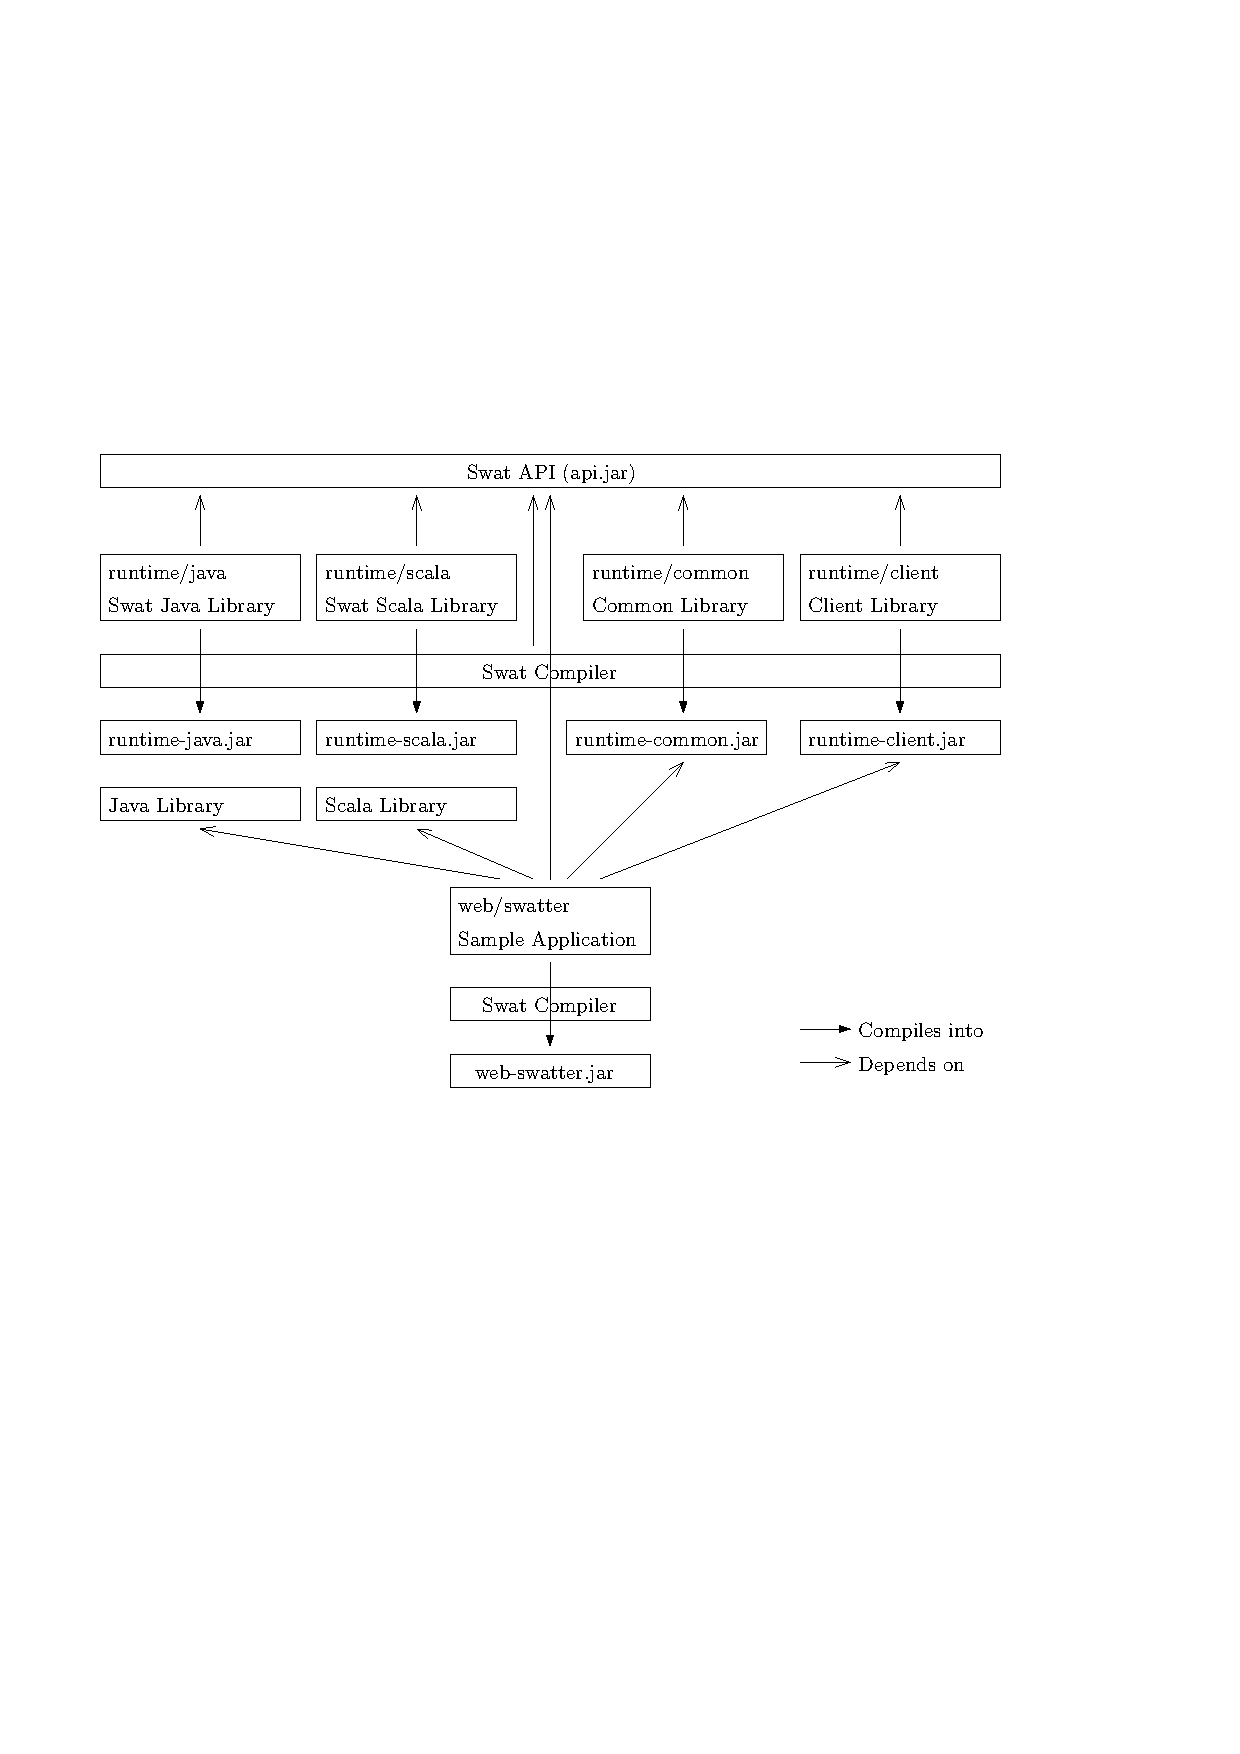
\includegraphics[width=\linewidth,height=\textheight,keepaspectratio]{img/Project.pdf}
	\caption{Runtime project compilation.}
	\label{Project}
\end{figure}

An application that should be compiled to JavaScript (e.g. \texttt{web/swatter}) depends on the \texttt{runtime/common} and \texttt{runtime/client} so the application can access additional APIs provided by the Swat runtime. It implicitly depends (as all Scala applications) on the Standard Scala Library and Java Class Library. It does not depend on the versions \texttt{runtime/java} and \texttt{runtime/scala} adjusted for Swat. Consequently all types defined in the application could be used even on the server side because they do not depend on the adjusted versions of standard libraries. Pupose of the adjusted versions is to store typefiles of standard Java and Scala types, because obviously the typefiles are not present in the standard libraries as they are not compiled with Swat compiler.

\section{API (package \texttt{swat.api})}

The \texttt{api} library is completely visible to users of the toolkit and contains means for interoperation with JavaScript environment and a few annotations that somehow affect the compilation process. The annotations are currently only two, the \texttt{swat.ingored} makes the Swat compiler completely ingore the annotated type, the \texttt{swat.adapter} informs the compiler that the annotated type is an adapter of JavaScript native object.

The most important part of the \texttt{api} are predefined adapters for native JavaScript APIs. The adapters are added in a lazy manner which means that a new adapter is added when there is a need for it. There are couple of predefined adapters that should more less cover the following JavaScript APIs:

\begin{itemize}
\item Document Object Model (DOM) Level 3 Core Specification.\\
http://www.w3.org/TR/2004/REC-DOM-Level-3-Core-20040407/
\item Document Object Model (DOM) Level 3 Events Specification.\\
http://www.w3.org/TR/DOM-Level-3-Events/
\item JavaScript Objects, Browser Objects and HTML DOM Element Objects.\\
http://www.w3schools.com/jsref/default.asp
\item Web Workers.\\
http://www.w3.org/TR/workers/
\end{itemize}

First thing to notice is that the adapters do not blindly copy the specifications because the specifications are in some cases redundant and contain duplicities. Usage of Scala which is great for abstraction of common functionality allows to define a new trait (with no counterpart in the specification) for the shared operations. The trait can later be mixed into all adapters that have the specified operations. The \texttt{swat.js.html.elements.InputLike} trait is an example of such approach. It defines interface that is shared among all form input HTML elements and is mixed into \texttt{Input}, \texttt{Select} and \texttt{TextArea} adapters.

The second interesting part is how the global scope is established. The global scope richness depends on a context in which JavaScript code is executed. If a script is being executed in the standard context (applies to all scripts inside a page) then it may access the \texttt{window} object or manipulate with the page. On the other hand if a script is being executed inside a web worker (analogue to a thread) then it is forbidden to access the \texttt{window}. So the object \texttt{swat.js.CommonScope} defines API that is availible in all execution contexts, \texttt{swat.js.DefaultScope} defines what is availible inside the default execution context and \texttt{swat.js.SharedWorkerScope} what is accessible in a web worker. The preferred way is to use the \texttt{swat.js.CommonScope} which ensures that the code works in all execution contexts. And only when it is required use a more specific global scope.

\section{Compiler (package \texttt{swat.compiler})}

The Swat compiler is implemented as a plugin (\texttt{SwatCompilerPlugin}) to the Scala compiler, so it follows the Scala compiler plugin design guidelines\cite{CompilerPlugins}. The plugin adds one phase to the standard set of compiler phases. When the phase is executed during compilation it does not modify the input Scala ASTs at all and delegates control to the JavaScript frontend (class \texttt{ScalaAstProcessor}) as it can be seen on the figure \ref{SwatCompiler}. Additionaly there is also the \texttt{SwatCompiler} which wraps the whole plugged Scala compiler, adds a programmer friendly interface thus it is possible to perform the compilation to JavaScript programmatically.

\begin{figure}[ht]
  \centering
	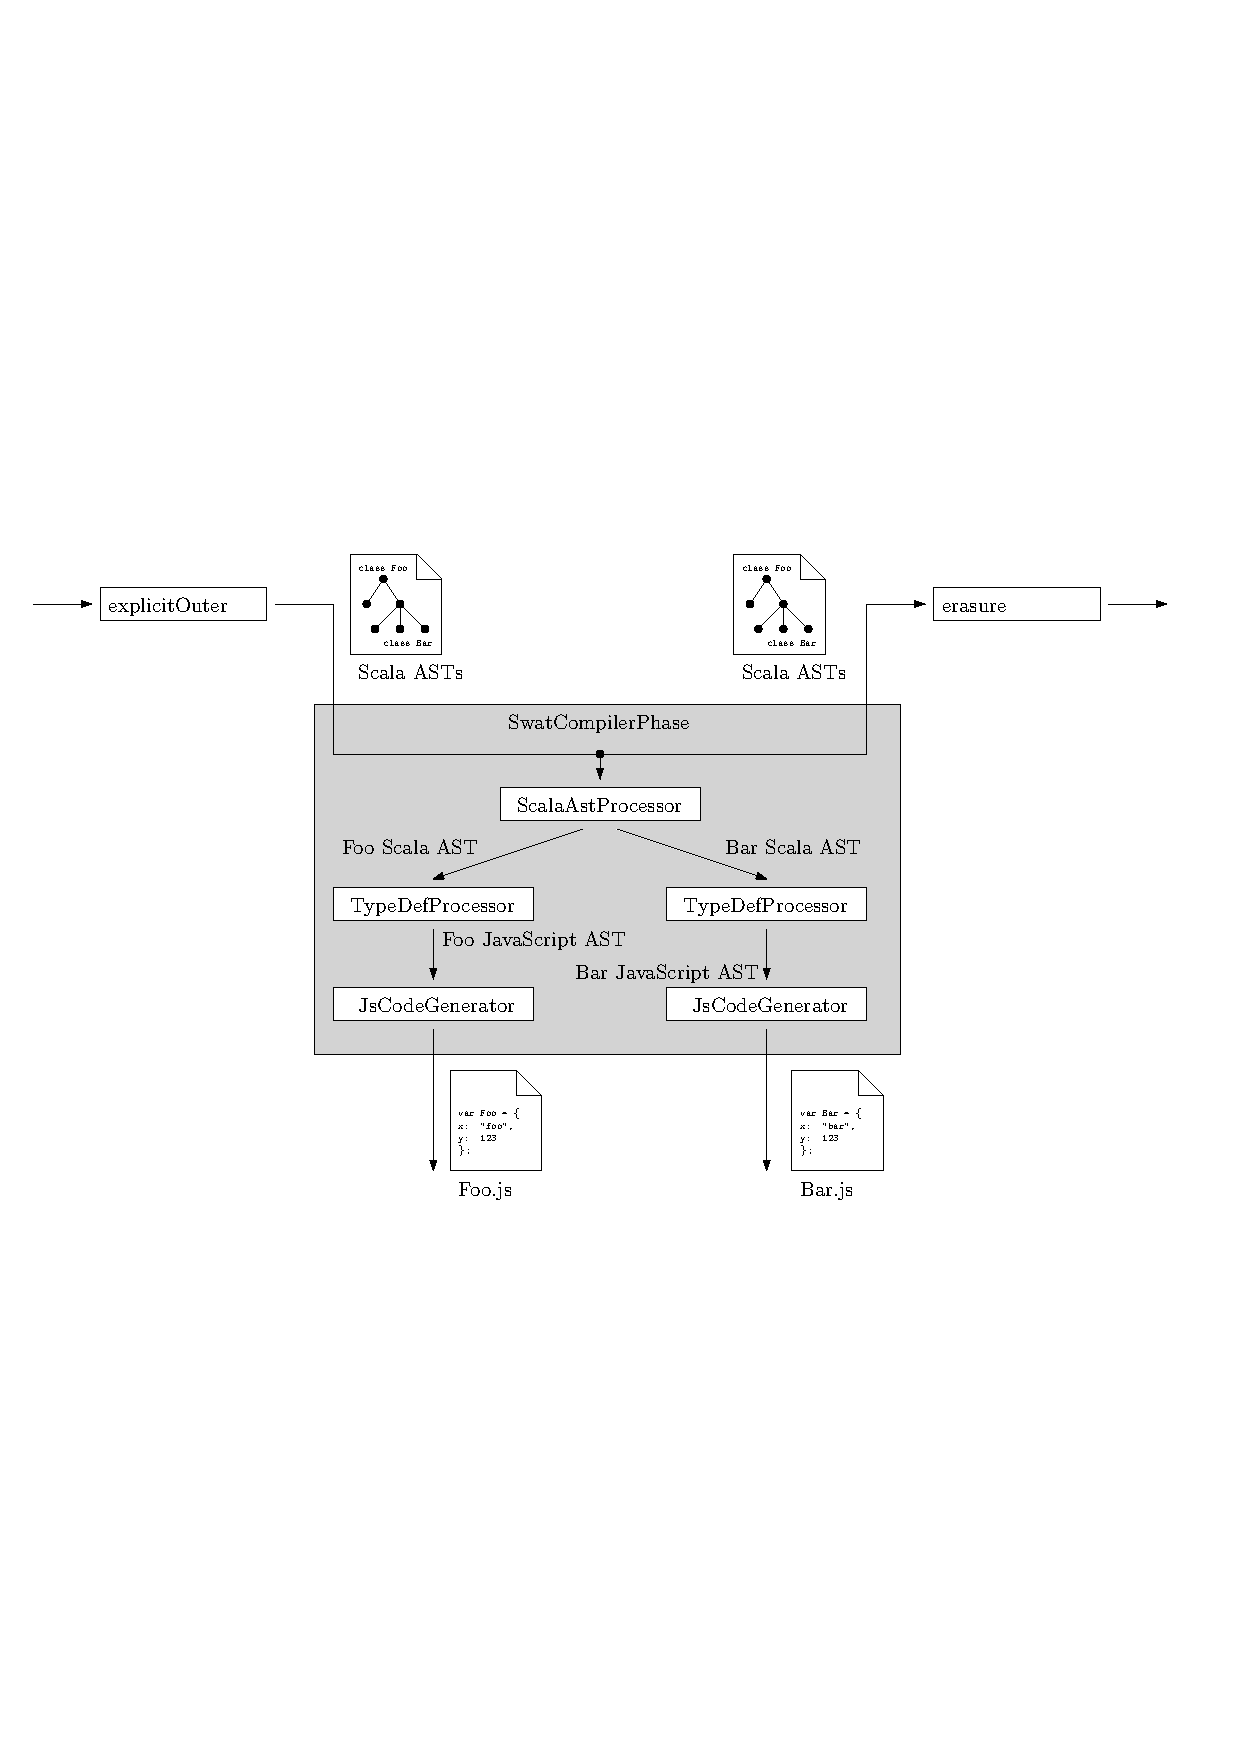
\includegraphics[width=\linewidth,height=\textheight,keepaspectratio]{img/SwatCompiler.pdf}
	\caption{Swat compiler implementation.}
	\label{SwatCompiler}
\end{figure}

There are three main subpackages: \texttt{js}, \texttt{frontend} and \texttt{backend}. The \texttt{js} package contains definitions of JavaScript ASTs and other syntax related constructs (e.g. keywords). The classes that represent syntax trees mirror the specification of JavaScript syntax\cite{EcmaScript} so any imaginable JavaScript program could be represented with these classes. In addition the \texttt{TreeBuilder} is a factory for some commonly used ASTs.

The \texttt{backend} package allows to generate JavaScript code from the ASTs. There is only one important class - \texttt{JsCodeGenerator}. From the top level point of view, it is just one big \texttt{match} expression against all types of ASTs where each \texttt{case} is responsible for one type. In most cases it works recursively becuase an AST is often composed of other ASTs. Therefore the encapsulated ASTs are processed first and then the resulting code fragments are somehow combined together.

\subsection{Frontend (package \texttt{swat.compiler.frontend})}

An entry point to the frontend is the \texttt{ScalaAstProcessor} class. Its functionality is pretty straightforward as it just traverses body of a \texttt{CompilationUnit} in order to find all type definitions. Then for each type definition it creates a new \texttt{TypeDefProcessor} and lets it process the type definition.

The \texttt{TypeDefProcessor} is an abstract class resposible for transformation of a type definition Scala ASTs to JavaScript ASTs. It defines functionality common for all kinds of type definitions and for each kind it has corresponding subclass: \texttt{ClassProcessor} for class definitions, \texttt{TraitProcessor} for trait definitions and \texttt{ObjectProcessor} for singleton object definitions. The subclasses are very simple, most of the functionality is shared and defined in the \texttt{TypeDefProcessor}.

An approach used inside the \texttt{TypeDefProcessor} is very similar to how the \texttt{JsCodeGenerator} generates JavaScript code, the main difference is that the \texttt{TypeDefProcessor} generates JavaScript ASTs. First of all, methods are extracted from the type definition, groupped by their names and processed as it is described in the {\it Analysis}. Processing a method group means that all overloaded variants are processed separately and then encoded to a single JavaScript AST representing the whole method group. The approach with a \texttt{match} against all Scala AST types is used for transformation of a method body. Only important thing is that it has to transform the ASTs according to {\it Analysis}, the rest are more less technical details that are not interesting in the context of the thesis. Finally when all the method groups are processed the type definition can be encoded into a single JavaScript AST containing the members, type name and linearized supertypes.


\section{Runtime}

\subsection{Client}

Description of everything intereseting in the swat.js.

\subsection{Standard Libraries}

Lazy approach, modifying the sources to exclude parts not relevant in the JavaScript environment. The purpose is not to blindly port everything but rather only a portion which is usable in JavaScript.

\subsection{Type Loader}

How it works on the server side and how on the client side.

\subsection{JSON Serializer}

The format that enables us to serialize even graphs of objects with cyclic references. Including type information in order to succesfully deserialize on the server and assign proper prototype on the client.

\subsection{RPC}

Support from the compiler, thin client proxy and server dispatcher. Only non-blocking, utilizing Scala Futures and Promises, exception handling.

\section{Integration with a Web Framework}

The Swat toolkit was designed with focus on simple integration to existing web application frameworks. The web application has to handle the following four HTTP requests which are used by the toolkit:

\begin{itemize}
\item \texttt{GET /swat/tpe/<typeIdentifier>}\\
Returns JavaScript code of the specified type.
\item \texttt{GET /swat/app/<typeIdentifier>/<args?>}\\
Returns JavaScript code of the specified type that mixes-in the \texttt{scala.App}. When executed in a browser the specified application starts running. The arguments are optional and allow simple parametrization of the application.
\item \texttt{POST /swat/rpc/<methodIdentifier>}\\
Returns result of the specified remote method invocation.  
\end{itemize}

For all those requests the Swat toolkit already defines complete implementation so the web application just has to forward such requests to Swat classes. An example integration to the Play MVC Framework\cite{Play} can be seen on the listing \ref{lst:PlayIntegration}. You may also notice that the toolkit uses Scala Futures\cite{ScalaFutures} so when an operation blocks on e.g. system operation, the thread may be used to handle another request. As a consequence scalability of the whole application increases.

\begin{lstlisting}[caption={Integration of Swat toolkit to Play Framework.},label={lst:PlayIntegration}	,basicstyle=\scriptsize\ttfamily,]
object Swat extends Controller {
    def tpe(typeIdentifier: String) = AsyncAction { r =>
        TypeLoader.getOrAlert(Array(typeIdentifier), Array.empty)
    }

    def app(typeIdentifier: String, args: String) = AsyncAction { r =>
        TypeLoader.getAppOrAlert(typeIdentifier, args.split(","))
    }

    def rpc(methodIdentifier: String) = AsyncAction { r =>
        val arguments = r.body.asJson.map(_.toString()).getOrElse("")
        RpcDispatcher.invoke(methodIdentifier, arguments)
    }

    private def AsyncAction(a: Request[AnyContent] => Future[String]) = Action { r =>
        Async(a(r).map(Ok(_)))
    }
}
\end{lstlisting}

\section{Build Process}

Integration with SBT was initially planned as a plugin to SBT. A user of the toolkit would specify that his solution requires the "Swat SBT plugin" which would allow him to define not only standard Scala projects but also "Swat projects". SBT would download the plugin from the internet during startup and the plugin would be responsible for invocation of the Swat compiler during compilation of a "Swat project". 

The proposed setup would be nice, however it turned out that SBT plugins have to be binary compatible with SBT itself (i.e. use same version of Scala as SBT). The proposed "Swat SBT plugin" would have to use Scala 2.10.1 because it invokes the Swat compiler which uses Scala 2.10.1 itself. On the other hand the latest version of SBT (at time of writing the thesis) uses Scala 2.9 and therefore the plugin would be incompatible with SBT.

It has been solved by a new SBT action: besides standard compilation action \texttt{compile} a new action \texttt{swat} is introduced. The \texttt{swat} action invokes the Swat compiler explicitly, but it is not that user friendly and compilation to JavaScript is not done in one step together with standard compilation. As soon as SBT comes out with Scala 2.10.1 build, the proposed plugin should be implemented and replace the temporary hack.

\section{Tests}

Most of the libraries in the toolkit are covered with tests with purpose to early detect bugs that can later be introduced. Especially the \texttt{compiler} tests are useful, because a simple modification that seems correct may actually break compilation of an AST when it is used in a different context. To run the tests start the SBT and execute the \texttt{test} action (i.e. write "test" and confirm it with enter).



%%%%%%%%%%%%%%%%%%%%%%%%%%%%%%%%%%%%%%%%%%%%%%%%%%%%%%%%%%%%%%%%%%%%%%%%%%%%%%%%
\chapter{Comparison with Similar Tools}

The tools at the time of thesis start (ScalaGWT, s2js, scalosure) and current scala-js, js-scala.



%%%%%%%%%%%%%%%%%%%%%%%%%%%%%%%%%%%%%%%%%%%%%%%%%%%%%%%%%%%%%%%%%%%%%%%%%%%%%%%%
\chapter{Conclusion}

\section{Critical Evaluation}

What was done, what lacks the most (Scala library), but stating that everything got done to some extent.

\section{Roadmap}

Actually the main purpose and goal is to really simplify tasks, that aren't programmer friendly in JavaScript. The grounds have been laid, so the really interesting applications can be now implemented. Some of the interesting directions are described in the following sections.

\subsection{Web workers}

Actor like abstraction over web workers, with help of JSON serializer and type-loader.

\subsection{Template Engine}

Problems with JavaScript templating and how it could be solved using string interpolation.

\subsection{Build Process}

Swat as a SBT plugin, resident compilation that would simplify the development process.



%%%%%%%%%%%%%%%%%%%%%%%%%%%%%%%%%%%%%%%%%%%%%%%%%%%%%%%%%%%%%%%%%%%%%%%%%%%%%%%%
\def\bibname{Bibliography}

\begin{thebibliography}{99}
\addcontentsline{toc}{chapter}{\bibname}

\bibitem{Flash}
	Introducing the Adobe Flash Platform.\\
	http://www.adobe.com/devnet/flashplatform/articles/flashplatform\_overview.html
	
\bibitem{JavaApplets}
	Java applet.\\
	http://en.wikipedia.org/wiki/Java\_applet
	
\bibitem{JavaScript}
	JavaScript.\\
	http://en.wikipedia.org/wiki/JavaScript
	
\bibitem{EcmaScript}
	{\sc Ecma} International.\\
	ECMAScript Language Specification.\\
	http://www.ecma-international.org/publications/files/ECMA-ST/Ecma-262.pdf
	
\bibitem{Ajax}
	{\sc Garrett,} Jesse James.\\
	Ajax: A New Approach to Web Applications.\\
	http://www.adaptivepath.com/ideas/ajax-new-approach-web-applications

\bibitem{Html5}
	HTML5 Introduction.\\
	http://www.w3schools.com/html/html5\_intro.asp

\bibitem{Backends}
  {\sc Ashkenas,} Jeremy.\\
  List of languages that compile to JS.\\
  https://github.com/jashkenas/coffee-script/wiki/List-of-languages-that-compile-to-JS
	
\bibitem{Meijer}
	{\sc Meijer,} Erik and {\sc Drayton,} Peter.\\
	Static Typing Where Possible, Dynamic Typing When Needed: The End of the Cold War Between Programming Languages.\\
	http://research.microsoft.com/en-us/um/people/emeijer/Papers/RDL04Meijer.pdf
	
\bibitem{RequireJs}
	RequireJS.\\
	http://requirejs.org/
	
\bibitem{HeadJs}
	HeadJS.\\
	http://headjs.com/
	
\bibitem{JsLint}
	JSLint, The JavaScript Code Quality Tool.\\
	http://www.jslint.com/
	
\bibitem{JsHint}
	JSHint, a JavaScript Code Quality Tool.\\
	http://www.jshint.com/

\bibitem{GoogleClosure}
	Google Closure Compiler.\\
	http://closure-compiler.appspot.com/home
	
\bibitem{Dart}
	Dart: Structured web apps.\\
	www.dartlang.org/
	
\bibitem{CoffeeScript}
	CoffeeScript.\\
	http://coffeescript.org/
	
\bibitem{TypeScript}
	TypeScript.\\
	www.typescriptlang.org/
	
\bibitem{NodeJs}
	node.js\\
	http://nodejs.org/
	
\bibitem{Rpc}
	Remote procedure call.\\
	http://en.wikipedia.org/wiki/Remote\_procedure\_call
	
\bibitem{Gwt}
	GWT Project.\\
	www.gwtproject.org/
	
\bibitem{SharpKit}
	SharpKit - C\# to JavaScript Compiler.\\
	http://sharpkit.net/
	
\bibitem{Tiobe}
	TIOBE Programming Community Index for July 2013.\\
	http://www.tiobe.com/index.php/content/paperinfo/tpci/index.html
	
\bibitem{Dom}
	Document Object Model (DOM) Specifications.\\
	http://www.w3.org/DOM/DOMTR
		
\bibitem{Jquery}
	jQuery.\\
	http://jquery.com/
	
\bibitem{Sbt}
	Scala Build Tool.\\
	http://www.scala-sbt.org/
	
\bibitem{Play}
	Play.\\
	http://www.playframework.com/
	
\bibitem{Typesafe}
	Typesafe.\\
	http://typesafe.com/
	
\bibitem{Self}
	Self.
	http://selflanguage.org/
	
\bibitem{ScalableComponents}
	{\sc Odersky,} Martin and {\sc Zenger,} Matthias.\\
	Scalable Component Abstractions.\\
	http://lampwww.epfl.ch/~odersky/papers/ScalableComponent.pdf
	
\bibitem{Linq}
  LINQ (Language-Integrated Query).\\
  http://msdn.microsoft.com/en-us/library/vstudio/bb397926.aspx
	
\bibitem{ScalaProgramming}
	{\sc Odersky,} Martin and {\sc Spoon,} Lex and {\sc Venners,} Bill.\\  Programming in Scala, Second Edition.\\
	Artima, 2010
	
\bibitem{ScalaAdvancedTypes}
	Advantages of Scala's Type System.\\
	http://stackoverflow.com/questions/3112725/advantages-of-scalas-type-system
	
\bibitem{Linearization}
  {\sc McBeath}, Jim.\\
	Scala Class Linearization.\\
	http://jim-mcbeath.blogspot.cz/2009/08/scala-class-linearization.html
	
\bibitem{Reflection}
	Symbols, Trees, and Types.\\
	http://docs.scala-lang.org/overviews/reflection/symbols-trees-types.html
	
\bibitem{SourceMaps}
  {\sc Seddon,} Ryan.\\
	Introduction to JavaScript Source Maps.\\
  http://www.html5rocks.com/en/tutorials/developertools/sourcemaps/
	
\bibitem{W3c}
  World Wide Web Consortium.\\
	http://www.w3.org/
	
\bibitem{ScalaDynamic}
  Scala Dynamic.\\
	http://www.scala-lang.org/api/current/index.html\#scala.Dynamic
	
\bibitem{ScalaLibrary}
	Scala Standard Library API.\\
  http://www.scala-lang.org/api/current/index.html\#package
	
\bibitem{Lazy}
  Lazy initialization.\\
	http://en.wikipedia.org/wiki/Lazy\_initialization
	
\bibitem{CompilerPlugins}
  Writing Scala Compiler Plugins.\\
  http://www.scala-lang.org/node/140
	
\bibitem{ScalaFutures}
  Futures and Promises.\\
  http://docs.scala-lang.org/overviews/core/futures.html
	
\bibitem{ScalaGwt}
  Scala+GWT Project.\\
  https://github.com/scalagwt
	
\bibitem{S2js}
  S2JS Compiler Plugin.\\
  https://github.com/alvaroc1/s2js
	
\bibitem{Scalosure}
  Scalosure.\\
  https://github.com/efleming969/scalosure
	
\bibitem{JsScala}
  js.scala: JavaScript as an embedded DSL in Scala.\\
  https://github.com/js-scala/js-scala
	
\bibitem{ScalaJs}
  Scala.js, a Scala to JavaScript compiler.\\
  https://github.com/sjrd/scala-js
	
\bibitem{WebWorkers}
  Using web workers.\\
  https://developer.mozilla.org/en-US/docs/Web/Guide/Performance/Using\_web\_workers
	
\bibitem{Actors}
  Actor Model.\\
  http://en.wikipedia.org/wiki/Actor\_model
	
\bibitem{Akka}
	akka.\\
	http://akka.io/
	
\bibitem{WebSockets}
  Introducing WebSockets: Bringing Sockets to the Web.\\
	http://www.html5rocks.com/en/tutorials/websockets/basics/
	
\bibitem{StringInterpolation}
  Scala Documentation.\\
	String Interpolation.\\
	http://docs.scala-lang.org/overviews/core/string-interpolation.html
	
\bibitem{Equality}
  {\sc Odersky,} Martin and {\sc Spoon,} Lex and {\sc Venners,} Bill.\\
  How to Write an Equality Method in Java.\\
	{sc}
	http://www.artima.com/lejava/articles/equality.html
	
\end{thebibliography}





%%%%%%%%%%%%%%%%%%%%%%%%%%%%%%%%%%%%%%%%%%%%%%%%%%%%%%%%%%%%%%%%%%%%%%%%%%%%%%%%
\appendix
\appendixpage
\addappheadtotoc

\chapter{User Manual}

\chapter{Sample Application}

A nice example could be online SWAT compiler, that would let the user write some Scala code to a textarea, invoke the Swat compiler (through RPC on the server) and display the compiler code.



%%%%%%%%%%%%%%%%%%%%%%%%%%%%%%%%%%%%%%%%%%%%%%%%%%%%%%%%%%%%%%%%%%%%%%%%%%%%%%%%
\chapter{Content of attached CD}





\printnomenclature




\end{document}
